%% ----------------------------------------------------------------
%% Thesis.tex -- MAIN FILE (the one that you compile with LaTeX)
%% ---------------------------------------------------------------- 

% Set up the document
\documentclass[a4paper, 11pt, oneside]{Thesis}  % Use the "Thesis" style, based on the ECS Thesis style by Steve Gunn
\graphicspath{{Figures/}}  % Location of the graphics files (set up for graphics to be in PDF format)

% Include any extra LaTeX packages required
\usepackage[square, numbers, comma, sort&compress]{natbib}  % Use the "Natbib" style for the references in the Bibliography
\usepackage{verbatim}  % Needed for the "comment" environment to make LaTeX comments
\usepackage{vector}  % Allows "\bvec{}" and "\buvec{}" for "blackboard" style bold vectors in maths
\hypersetup{urlcolor=blue, colorlinks=true}  % Colours hyperlinks in blue, but this can be distracting if there are many links.

%% ----------------------------------------------------------------
\begin{document}
\frontmatter      % Begin Roman style (i, ii, iii, iv...) page numbering

% Set up the Title Page
\title  {Data Driven Automated Algorithmic Trading}
\authors  {\texorpdfstring
            {\href{gabriel@gaucimaistre.com}{Gabriel Gauci Maistre}}
            {Gabriel Gauci Maistre}
            }
\addresses  {\groupname\\\deptname\\\univname}  % Do not change this here, instead these must be set in the "Thesis.cls" file, please look through it instead
\date       {\today}
\subject    {}
\keywords   {}

\maketitle
%% ----------------------------------------------------------------

\setstretch{1.3}  % It is better to have smaller font and larger line spacing than the other way round

% Define the page headers using the FancyHdr package and set up for one-sided printing
\fancyhead{}  % Clears all page headers and footers
\rhead{\thepage}  % Sets the right side header to show the page number
\lhead{}  % Clears the left side page header

\pagestyle{fancy}  % Finally, use the "fancy" page style to implement the FancyHdr headers

%% ----------------------------------------------------------------
% Declaration Page required for the Thesis, your institution may give you a different text to place here
\Declaration{

\addtocontents{toc}{\vspace{1em}}  % Add a gap in the Contents, for aesthetics

I, Gabriel Gauci Maistre, declare that this thesis titled, `Data Driven Automated Algorithmic Trading' and the work presented in it are my own. I confirm that:

\begin{itemize} 
\item[\tiny{$\blacksquare$}] This work was done wholly or mainly while in candidature for a research degree at this University.
 
\item[\tiny{$\blacksquare$}] Where any part of this thesis has previously been submitted for a degree or any other qualification at this University or any other institution, this has been clearly stated.
 
\item[\tiny{$\blacksquare$}] Where I have consulted the published work of others, this is always clearly attributed.
 
\item[\tiny{$\blacksquare$}] Where I have quoted from the work of others, the source is always given. With the exception of such quotations, this thesis is entirely my own work.
 
\item[\tiny{$\blacksquare$}] I have acknowledged all main sources of help.
 
\item[\tiny{$\blacksquare$}] Where the thesis is based on work done by myself jointly with others, I have made clear exactly what was done by others and what I have contributed myself.
\\
\end{itemize}
 
 
Signed:\\
\rule[1em]{25em}{0.5pt}  % This prints a line for the signature
 
Date:\\
\rule[1em]{25em}{0.5pt}  % This prints a line to write the date
}
\clearpage  % Declaration ended, now start a new page

%% ----------------------------------------------------------------
% The "Funny Quote Page"
\pagestyle{empty}  % No headers or footers for the following pages

\null\vfill
% Now comes the "Funny Quote", written in italics
\textit{``If past history was all there was to the game, the richest people would be librarians.''}

\begin{flushright}
Warren Buffett
\end{flushright}

\vfill\vfill\vfill\vfill\vfill\vfill\null
\clearpage  % Funny Quote page ended, start a new page
%% ----------------------------------------------------------------

% The Abstract Page
\addtotoc{Abstract}  % Add the "Abstract" page entry to the Contents
\abstract{
\addtocontents{toc}{\vspace{1em}}  % Add a gap in the Contents, for aesthetics

Various existing stock market price forecasting methods were analysed in this report. Three methods were applied towards the problem making use of Technical Analysis, these were Time Series Analysis, Machine Learning, and Bayesian Statistics. Through the results of this report, it was found that the Efficient Market Hypothesis remains true, that past data does not contain enough useful information to forecast future prices and gain an advantage over the market. However, the results proved that Technical Analysis and Machine Learning could still be used to guide an investor’s decision. It was also found that the Random Walk Hypothesis was not necessarily true, as some stocks showed signs of auto and partial correlation. A common application of technical analysis was demonstrated and shown to produce limited useful information in beating the market. Based on the findings, a number of automated trading algorithms were developed using machine learning and backtested to determine their effectiveness.

}

\clearpage  % Abstract ended, start a new page
%% ----------------------------------------------------------------

\setstretch{1.3}  % Reset the line-spacing to 1.3 for body text (if it has changed)

% The Acknowledgements page, for thanking everyone
\acknowledgements{
\addtocontents{toc}{\vspace{1em}}  % Add a gap in the Contents, for aesthetics

I would like to express my special thanks of gratitude to my supervisor, Alan Gatt, for the patient guidance, encouragement, and advice he has provided throughout my time as his student.

I would also like to thank Luke Vella Critien, for guiding me towards the right parth in the early stages of my research and for recommending Alan Gatt as my tutor. 

My gratitude is also extended to Emma Galea and Miguel attard for their valuable input while carrying out my research.

Completing this work would have been all the more difficult were it not for the support and friendship provided by the other members of the Malta College of Arts, Sciences, and Technology, and the institute of Information and Technology. I am indebted to them for their help.

Finally, I would like to thank my family who have supported me all throughout the final year of my bachelor's.

}
\clearpage  % End of the Acknowledgements
%% ----------------------------------------------------------------

\pagestyle{fancy}  %The page style headers have been "empty" all this time, now use the "fancy" headers as defined before to bring them back


%% ----------------------------------------------------------------
\lhead{\emph{Contents}}  % Set the left side page header to "Contents"
\tableofcontents  % Write out the Table of Contents

%% ----------------------------------------------------------------
\lhead{\emph{List of Figures}}  % Set the left side page header to "List if Figures"
\listoffigures  % Write out the List of Figures

%% ----------------------------------------------------------------
\lhead{\emph{List of Tables}}  % Set the left side page header to "List of Tables"
\listoftables  % Write out the List of Tables

%% ----------------------------------------------------------------
\setstretch{1.5}  % Set the line spacing to 1.5, this makes the following tables easier to read
\clearpage  % Start a new page
\lhead{\emph{Abbreviations}}  % Set the left side page header to "Abbreviations"
\listofsymbols{ll}  % Include a list of Abbreviations (a table of two columns)
{
% \textbf{Acronym} & \textbf{W}hat (it) \textbf{S}tands \textbf{F}or \\
\textbf{EMH} & \textbf{E}fficient \textbf{M}arket \textbf{H}ypothesis \\
\textbf{RWH} & \textbf{R}andom \textbf{W}alk \textbf{H}ypothesis \\
\textbf{OLS} & \textbf{O}rdinary \textbf{L}east \textbf{S}quares \\
\textbf{AR} & \textbf{A}uto \textbf{R}egressive \\
\textbf{MA} & \textbf{M}oving \textbf{A}verage \\
\textbf{ARMA} & \textbf{A}uto \textbf{R}egressive \textbf{M}oving \textbf{A}verage \\
\textbf{ARIMA} & \textbf{A}uto \textbf{R}egressive \textbf{I}ntegrated \textbf{M}oving \textbf{A}verage \\
\textbf{GARCH} & \textbf{G}eneralised \textbf{A}uto \textbf{R}egressive \textbf{C}onditional \textbf{H}eteroskedasticity \\
\textbf{EGARCH} & \textbf{E}xponential \textbf{G}eneralised \textbf{A}uto \textbf{R}egressive \textbf{C}onditional \textbf{H}eteroskedasticity \\
\textbf{ADF} & \textbf{A}ugmented \textbf{D}ickey \textbf{F}uller \\
\textbf{SVM} & \textbf{S}upport \textbf{V}ector \textbf{M}achine \\
\textbf{SGD} & \textbf{S}tochastic \textbf{G}radient \textbf{D}escent \\
\textbf{SMA} & \textbf{S}imple \textbf{M}oving \textbf{A}verage \\
\textbf{AIC} & \textbf{A}lkaline \textbf{I}nformation \textbf{C}riterion \\
\textbf{IC} & \textbf{I}nformation \textbf{C}riterion \\
\textbf{NUTS} & \textbf{N}o-\textbf{U}-\textbf{T}urn \textbf{S}ampler \\
\textbf{QQ} & \textbf{Q}uantile-\textbf{Q}uantile \\
\textbf{ETF} & \textbf{E}xchange \textbf{T}raded \textbf{F}und \\
\textbf{ANN} & \textbf{A}rtificial \textbf{N}eural \textbf{N}etwork
}

%% ----------------------------------------------------------------
% End of the pre-able, contents and lists of things
% Begin the Dedication page

\setstretch{1.3}  % Return the line spacing back to 1.3

\pagestyle{empty}  % Page style needs to be empty for this page
\lhead{\emph{Dedicatory}}  % Set the left side page header to "Symbols"
\dedicatory{To my parents, Keith \& Christine Gauci Maistre. Without them, and their unconditional love and support, none of this would have been possible.}

\addtocontents{toc}{\vspace{2em}}  % Add a gap in the Contents, for aesthetics


%% ----------------------------------------------------------------
\mainmatter	  % Begin normal, numeric (1,2,3...) page numbering
\pagestyle{fancy}  % Return the page headers back to the "fancy" style

% Include the chapters of the thesis, as separate files
% Just uncomment the lines as you write the chapters

\lhead{\emph{Introduction}}  % Set the left side page header to "Symbols"
\chapter{Introduction}

"Investing in stocks is just like gambling" - is a phrase commonly heard coming from people describing stock investing. But is it really just like gambling? Were all those investors who made billions from the stock market just lucky? To understand this, we must first review what it means to buy stocks. In the stock market, buying stocks means owning a share of the company. It entitles the stock holder to a claim on assets as well as a fraction of the profits which the company generates. It is unfortunately very common for investors to misunderstand this concept, often thinking of shares as simply a trading vehicle and forget that stock represents the ownership of a company. 

So how are stocks valued? The value of a company’s stock depends on a number of factors, and assessing the value is not an easy practice. Investors are constantly trying to assess the profit that will be left over to shareholders. This is why stock prices fluctuate. The outlook for business conditions is always changing, and so are the future earnings of a company. Since many people fail to understand this concept, it is far too common to believe that the short-term price movements of a company are random. However, it is the long-term price movements of a company which reflect the value of a company as it is supposed to be worth the present value of the profits it will make. A company can survive without profits in the short term, as long as expectations of future earnings exist. A company may try to fool investors in the beginning, however a company’s stock price will eventually be expected to show the true value of the firm.

So how is this all different to gambling? Gambling is a zero-sum game. It merely takes money from a loser and gives it to a winner. No value is ever created. By investing, we increase the overall wealth of an economy. As companies compete, they increase productivity and develop products that can make our lives better. This does not mean that stock investing cannot be a gamble, as it is extremely common for many people to skip the due diligence before spending a huge chunk of their life savings on stock, often losing it all in the process.

This report aims to disprove three hypotheses, the Efficient Market Hypotheses (EMH), the Zero-Sum Game theory, and the Random Walk Hypothesis.

\section{Efficient Market Hypothesis - EMH}

In financial economics, the efficient market hypothesis (EMH) is an investment theory which states it is impossible for an investor to "beat the market" because stock market efficiency causes existing share prices to always incorporate and reflect all relevant information. In accordance to the EMH, stocks always trade at their fair value on stock exchanges and only react to new information or charges in discount rates, making it impossible for investors to make a profit by either purchasing undervalued stocks or selling stocks for inflated prices. This means that as such, it should be impossible to outperform the overall market through expert stock selection or market timing, and the only way an investor can possibly obtain higher returns is by purchasing riskier investments.

\subsection{Breaking down EMH}
Although it is a cornerstone of modern financial theory, the EMH is highly controversial and often disputed. Believers argue it is pointless to search for undervalued stocks or to try to predict trends in the market through either fundamental or technical analysis.

While academics point to a large body of evidence in support of EMH, an equal amount of dissension also exists. For example, investors such as Warren Buffett have consistently beaten the market over long periods of time, which  in itself is impossible by definition according to the EMH. Detractors of the EMH also point to events such as the 1987 stock market crash, when the Dow Jones Industrial Average (DJIA) fell by over 20\% in a single day, which was clear evidence that stock prices can seriously deviate from their fair values.

Proponents of the EMH conclude that, because of the randomness of the market, investors would be better off by investing in a low-cost, passive portfolio such as one comprising of various low risk index funds. Data compiled by Morningstar Inc. through its June 2015 Active/Passive Barometer study supports the conclusion. Morningstar compared active managers’ returns in all categories against a composite made of related index funds and exchange-traded funds (ETFs). The study found that year-over-year, only two groups of active managers successfully outperformed passive funds more than 50\% of the time. These were U.S. small growth funds and diversified emerging markets funds.

In all of the other categories, including U.S. large blend, U.S. large value, and U.S. large growth, among others, investors would have fared better by investing in low-cost index funds or ETFs. While a percentage of active managers do outperform passive funds at some point, the challenge for investors is being able to identify which ones will do so. Less than 25\% of the top-performing active managers are able to consistently outperform their passive manager counterparts.

\section{Zero-Sum Game}
Zero-sum, not to be confused with Empty sum, or Zero game, is a mathematical representation of a situation found in game theory and economic theory, in which one person’s gain is equivalent to another’s loss, so the net change in wealth or benefit is zero. A zero-sum game may have as few as two players, or millions of participants.

Zero-sum games are found in game theory, but are less common than non-zero sum games. Poker and gambling are popular examples of zero-sum games since the sum of the amounts won by some players equals the combined losses of the others. Games such as chess and tennis, in which there is one winner and one loser, are also zero-sum games.

It is important to note that the stock market overall is often considered a zero-sum game, which is a misconception, along with other popular misunderstandings. Historically and in contemporary culture the stock market is often equated with gambling, which is definitely a zero-sum game. When an investor buys a stock, it is a share of ownership of a company that entitles that investor to a fraction of the company's profits. The value of a stock can go up or down depending on the economy and a host of other factors, but ultimately, ownership of that stock will eventually result in a profit or a loss that is not based on chance or the guarantee of someone else's loss. In contrast, gambling means that somebody wins the money of another who loses it.

\section{Random Walk Hypothesis}
The random walk theory suggests that stock price changes have the same distribution and are independent of each other, so the past movement or trend of a stock price or market cannot be used to predict its future movement. In short, this is the idea that stocks take a random and unpredictable path.

A follower of the random walk theory believes it's impossible to outperform the market without assuming additional risk. Critics of the theory, however, contend that stocks do maintain price trends over time – in other words, that it is possible to outperform the market by carefully selecting entry and exit points for equity investments. % Introduction

\lhead{\emph{Background Theory}}  % Set the left side page header to "Symbols"
\chapter{Background Theory}

Computational finance is a branch of applied computer science that deals with problems of practical interest in finance. Some slightly different definitions are the study of data and algorithms currently used in finance and the mathematics of computer programs that realize financial models or systems. Using computational finance in order to allocate assets in a portfolio is not at all unheard of and was first documented  1952.\cite{Markowitz:1952aa} Markowitz first introduced the concept of portfolio selection as an exercise in mean-variance optimisation. This required more computer power than was available at the time, so he worked on useful algorithms for approximate solutions. He theorised that risk-averse investors could construct portfolios to optimise or maximise expected return based on a given level of market risk, emphasising that risk is an inherent part of higher reward. According to his theory, it's possible to construct an "efficient frontier" of optimal portfolios offering the maximum possible expected return for a given level of risk. 

\section{Time Series Analysis}

A time series is a series of data points which may be indexed, listed, or graphed, in a time order. Most commonly, a time series is a sequence taken at successive equally spaced points in time. Thus it is a sequence of discrete-time data. Examples of time series are heights of ocean tides, counts of sunspots, and the daily closing value of the Dow Jones Industrial Average. Brockwell et al provide a formal description of time series as having a set of observations xt, each one being recorded at a specific time t. A discrete-time time series (the type to which this book is primarily devoted) is one in which the set T0 of times at which observations are made is a discrete set, as is the case, for example, when observations are made at fixed time intervals. Continuous time series are obtained when observations are recorded continuously over some time interval, e.g., when T0 = [0, 1].\cite{Peter-J.-Brockwell:2016aa}

Significant "time series momentum" has also been documented in equity index, currency, commodity, and bond futures for each of the 58 liquid instruments they consider.\cite{Moskowitz:2011aa} They find persistence in returns for 1 to 12 months that partially reverses over longer horizons, consistent with sentiment theories of initial under-reaction and delayed over-reaction. A diversified portfolio of time series momentum strategies across all asset classes delivers substantial abnormal returns with little exposure to standard asset pricing factors and performs best during extreme markets. Examining the trading activities of speculators and hedgers, they find that speculators profit from time series momentum at the expense of hedgers.

\subsection{Auto Regressive Moving Average (ARMA)}

In the statistical analysis of time series, autoregressive–moving-average (ARMA) models provide a parsimonious description of a weakly stationary stochastic process in terms of two polynomials, one for the autoregression and the second for the moving average. The notation ARMA(p, q) refers to the model with p autoregressive terms and q moving-average terms. This model contains the AR(p) and MA(q) models,

\(x_t = c+\varepsilon_t+\sum^{q}_{i=1} \varphi_iX_{t-i}\theta_i\varepsilon_{t-i}\)

Forecasting interest rates is of great concern for financial researchers, economists, and players in the fixed income markets. A study was carried out to develop an appropriate model for forecasting the short-term interest rates, implicit yield on 91 day treasury bill, overnight MIBOR rate, and call money rate.\cite{Radha:2015aa} The short-term interest rates are forecasted using univariate models such as the Random Walk, ARIMA, ARMA-GARCH, and ARMA-EGARCH. The appropriate model for forecasting is determined considering a six-year period from 1999. The results show that interest rates time series have volatility clustering effect and hence GARCH based models are more appropriate to forecast than the other models. Radha et al found that for commercial paper rate ARIMA-EGARCH model is the most appropriate model, while for implicit yield 91 day Treasury bill, overnight MIBOR rate, and call money rate, the ARIMA-GARCH model is the most appropriate model for forecasting.

\subsection{Auto Regressive Integrated Moving Average (ARIMA)}

In time series analysis, an autoregressive integrated moving average (ARIMA) model is a generalization of an ARMA model. Given a time series of data $X_t$ where t is an integer index and the $X_t$ are real numbers, an ARMA(p, q) model is given by

\(x_t - \alpha_1 X_{t-1} - \dots \alpha_{p'} X_{t-p'} = \varepsilon_t + \theta_1 \epsilon_{t-1} + \dots + \theta_q \epsilon_{t-q}\)

The aforementioned model is fitted to time series data either to better understand the data or to predict future points in the series (forecasting). ARIMA models are applied in some cases where data show evidence of non-stationarity, where an initial differencing step (corresponding to the "integrated" part of the model) can be applied to reduce the non-stationarity. 

The existence of weak-form efficiency in the Russian stock market is examined for the period 1st September 1995 to 1st May 2001 using daily, weekly and monthly Russian Trading System index time series.\cite{Abrosimova:2002aa} Several different approaches are used to assess the predictability of the RTS index time series. Unit root, autocorrelation and variance ratio tests are conducted for the null hypothesis of a random walk model. The results support the null hypothesis for the monthly data only. Further analysis is performed for the daily and weekly data. Linear and non-linear modelling of the serial dependence is conducted using ARIMA and GARCH models estimated on the in-sample period 1st September 1995 to 1st January 2001. Forecasts based on the best fitting models are performed for the out-of-sample period 2nd January 2001 to 1st May 2001. Comparisons of the forecasts reveal that none of the models outperforms the others, and the most accurate forecasts are obtained for just the first out-of-sample observation. Whilst our research results provide some limited evidence of short-term market predictability on the RTS, there is insufficient evidence to suggest that it would lead to a profitable trading rule, once transaction costs and risk are taken into account.

The main intention of this paper is to investigate, with new daily data, whether prices in the two Chinese stock exchanges (Shanghai and Shenzhen) follow a random-walk process as required by market efficiency.\cite{Darrat:2001aa} We use two different approaches, the standard variance-ratio test of Lo and MacKinlay (1988) and a model-comparison test that compares the ex post forecasts from a NAIVE model with those obtained from several alternative models (ARIMA, GARCH and Artificial Neural Network-ANN). To evaluate ex post forecasts, we utilize several procedures including RMSE, MAE, Theil's U, and encompassing tests. In contrast to the variance-ratio test, results from the model-comparison approach are quite decisive in rejecting the random-walk hypothesis in both Chinese stock markets. Moreover, our results provide strong support for the ANN as a potentially useful device for predicting stock prices in emerging markets.

\section{Statistical Machine Learning}

A machine learning algorithm is an algorithm that is able to learn through examples from data. To understand what an algorithm is, Cormen et al informally describe algorithms as "any well-defined computational procedures which takes some value, or set of values, as input and produce some value, or set of values, as output. An algorithm is thus a sequence of computational steps that transform the input into the output."\cite{Cormen:2009aa} In simple terms, it is possible to say that an algorithm is a sequence of steps which allow to solve a certain task. Similarly to a normal algorithm, a machine learning algorithm as defined formally by Tom M. Mitchell, states that "A computer program is said to learn from experience E with respect to some class of tasks T and performance measure P, if its performance at tasks in T, as measured by P, improves with experience E."\cite{Mitchell:1997aa}

\subsection{Classification}

Classifiers are a class of machine learning algorithms which identify in which category a new observation belongs to, on the basis of a training set of data containing observations whose category membership is known. A model based on discriminant analysis was sought out to categorise a stock as manipulated or non-manipulated based on certain key variables that capture the characteristics of the stock.\cite{Murugesan:2012aa} The model in which Murugesan et al chose, helps them identify stocks witnessing activities that are indicative of potential manipulation irrespective of the type of manipulation, such as action-based, information-based, or trade-based. The model which they proposed, helps investigators to arrive at a shortlist of securities that are potentially manipulated and which could be subject to further detailed investigation to detect the type and nature of the manipulation, if any. In a market like India, where there are about 5000 plus securities listed on its major exchanges, it becomes extremely difficult to monitor all securities for potential market abuse. Academics who have earlier used discriminant analysis have used the Linear Classification Function without validating the assumption that governs the model. Through their research, they have tested the assumption on data from the Indian capital market and found that the data does not comply with the assumptions that govern the use of the linear classification function. This therefore resulted in them using the Quadratic Classification Function, which is the appropriate technique for instances where the data does not meet the sated assumptions, to categorise stocks into two categories, namely manipulated and non-manipulated.

\subsection{Support Vector Machines}

Support vector machines (SVM), are a class of machine learning algorithms that have become incredibly popular in the past few years. SVMs are very similar to classifiers in the sense that they also classify data by drawing a line, called a decision boundary, to separate them. However, SVMs go a step further by calculating a vector from the data point with the smallest margin to the decision boundary. This is called a support vector. There exists vast research articles which predict the stock market as well pricing of stock index financial instruments but most of the proposed models focus on the accurate forecasting of the levels of the underlying stock index. There is a lack of studies examining the predictability of the direction of stock index movement. Given the notion that a prediction with little forecast error does not necessarily translate into capital gain, the authors of this research attempt to predict the direction of the S\&P CNX NIFTY Market Index of the National Stock Exchange, one of the fastest growing financial exchanges in developing Asian countries.\cite{Kumar:2016aa} Random forest and Support Vector Machines (SVM) are very specific type of machine learning method, and are promising tools for the prediction of financial time series. The tested classification models, which predict direction, include linear discriminant analysis, logit, artificial neural network, random forest, and SVM. Empirical experimentation suggests that the SVM outperforms the other classification methods in terms of predicting the direction of the stock market movement and random forest method outperforms neural network, discriminant analysis and logit model used in their study.

\subsection{Regression}

Regression analysis is widely used for prediction and forecasting to understand which among the independent variables are related to the dependent variable while also exploring the forms of these relationships. In restricted circumstances, regression analysis can be used to infer causal relationships between the independent and dependent variables. Regression analysis helps one understand how the typical value of the dependent variable changes when any one of the independent variables is varied, while the other independent variables are held fixed. Kakushadze et al provide a systematic quantitative framework in what is intended to be a “pedagogical” fashion for discussing mean-reversion and optimisation.\cite{Kakushadze:2015aa} In their paper, they start off their research with pair trading and add complexity by following the sequence “mean-reversion via demeaning, regression, weighted regression, (constrained) optimization, factor models”. They discuss in further detail how to conduct mean-reversion based on this approach, including common pitfalls encountered in practical applications, such as the difference between maximising the Sharpe ratio and minimising an objective function when trading costs are included. Kakushadze et al also discuss explicit algorithms for optimization with linear costs, constraints and bounds, and also illustrate their discussion on an explicit intraday mean-reversion alpha.

\subsection{Decision Trees}

Decision tree learning uses a decision tree as a predictive model which maps observations about an item, represented in the branches, to conclusions about the item's target value represented in the leaves. Tree models where the target variable can take a finite set of values are called classification trees; in these tree structures, leaves represent class labels and branches represent conjunctions of features that lead to those class labels. Decision trees where the target variable can take continuous values, typically real numbers, are called regression trees. Creamer et al propose a multi-stock automated trading system which relies on a layered structure consisting of a machine learning algorithm, an online learning utility, and a risk management overlay.\cite{Creamer:2010aa} An alternating decision tree (ADT), which is implemented with Logitboost, was chosen as their underlying algorithm. One of the strengths of their approach is that the algorithm is able to select the best combination of rules derived from well-known technical analysis indicators and is also able to select the best parameters of the technical indicators. Additionally, their online learning layer combines the output of several ADTs and suggests a short or long position. Finally, the risk management layer in which they implemented, can validate the trading signal when it exceeds a specified non-zero threshold and limit the application of their trading strategy when it is not profitable. They tested the expert weighting algorithm with data of 100 randomly selected companies of the S\&P 500 index during the period 2003–2005. They found that their algorithm generates abnormal returns during the test period. Their experiments show that the boosting approach was able to improve the predictive capacity when indicators were combined and aggregated as a single predictor. Even more, the combination of indicators of different stocks demonstrated to be adequate in order to reduce the use of computational resources, and still maintain an adequate predictive capacity.

\section{Bayesian Statistics}

Bayesian Statistics, a form of probabilistic programming, describes probabilistic models and then performs inference in those models. Probabilistic reasoning is a foundational technology of machine learning and has been used by companies such as Google, Amazon, and Microsoft. Probabilistic reasoning has been used for predicting stock prices, recommending movies, diagnosing computers, detecting cyber intrusions, and image detection. Gelman et al defines bayesian inference as the process of fitting a probability model to a set of data and summarising the result by a probability distribution on the parameters of the model and on unobserved quantities such as predictions for new observations.\cite{Gelman:2014aa}

\subsection{Markov Chain Monte Carlo}

In statistics, Markov chain Monte Carlo (MCMC) methods are a class of algorithms for sampling from a probability distribution based on constructing a Markov chain that has the desired distribution of its equilibrium distribution. The state of the chain after a number of steps is then used as a sample of the desired distribution. The quality of the sample improves as a function of the number of steps.

A 1993 paper was prepared for the purpose of presenting the methodology and uses of the Markov Chain Monte Carlo simulation technique as applied in the evaluation of investment projects to analyse and assess risk.\cite{Savvides:1994aa} In the first part of his paper, he highlights the importance of risk analysis in investment appraisal. The author follows by presenting the various stages in the application of the risk analysis process and examines the interpretation of the results generated by a risk analysis application including investment decision criteria and various measures of risk based on the expected value concept. In the final part of his paper, he draws some conclusions regarding the usefulness and limitations of risk analysis in investment appraisal.

Stochastic volatility models are increasingly important in practical derivatives pricing applications, yet relatively little work has been undertaken in the development of practical Monte Carlo simulation methods for this class of models. This paper considers several new algorithms for time-discretization and Monte Carlo simulation of Heston-type stochastic volatility models.\cite{Andersen:2007aa} The algorithms are based on a careful analysis of the properties of affine stochastic volatility diffusions, and are straightforward and quick to implement and execute. Tests on realistic model parameterizations reveal that the computational efficiency and robustness of the simulation schemes proposed in the paper compare very favourably to existing methods.

Bond yields today are well below and stock market valuations are well above their historical average.\cite{Blanchett:2013aa} There are no historical periods in the United States where comparable low bond yields and high equity valuations have occurred simultaneously. Both current bond yields and stock values have been shown to predict near-term returns. Portfolio returns in the first decade of retirement have an outsize impact on retirement income strategies. Traditional Monte Carlo simulation approaches generally do not incorporate market valuations into their analysis. In order to simulate how retirees will fare in a low return environment for both stocks and bonds, Blanchett et al incorporate the predictive ability of current valuations to simulate its impact on retirement portfolios. Blanchett et al estimate bond returns through an autoregressive model that uses an initial bond yield value where yields drift in the future. Blanchett et al use the cyclically adjusted price-to-earnings (CAPE) ratio as an estimate of market valuation to predict short-run stock performance. Our simulations indicate that the safety of a given withdrawal strategy is significantly affected by the initial bond yield and CAPE value at retirement, and that the relative impact varies based on the portfolio equity allocation. Using valuation measures current as of April 15, 2013, which is a bond yield of 2.0\% and a CAPE of 22, Blanchett et al find the probability of success for a 40\% equity allocation with a 4\% initial withdrawal rate over a 30 year period is approximately 48\%. This success rate is materially lower than past studies and has sobering implications on the likelihood of success for retirees today, as well as how much those near retirement may need to save to ensure a successful retirement.

This paper provides a numerical approach based on a Monte Carlo simulation for valuing dynamic capital budgeting problems with many embedded real options dependent on numerous state variables.\cite{Gamba:2003aa} Schwartz et al propose a way of decomposing a complex capital budgeting problem with many options into a set of simple options, suitably accounting for interaction and interdependence among them. The decomposition approach is numerically implemented using an extension of the Least Squares Monte Carlo algorithm, presented by Longstaff and Schwartz (2001) applied to our multi-option setting. Schwartz et al also provide a number of applications of our approach to well-known real options models and real life capital budgeting problems. Moreover, Schwartz et al present a set of numerical experiments to provide evidence for the accuracy of the proposed methodology. % Background Theory 

\lhead{\emph{Experimental Setup}}  % Set the left side page header to "Symbols"
\chapter{Experimental Setup}

\section{Data Tidying}
A data set containing end of day stock prices, dividends, and splits for 3,000 US companies, curated by the Quandl community, and released into the public domain, was used. The date column in the CSV file was loaded into memory, and said column was converted to a date data type. The DataFrame was then sorted using the date column, starting from the oldest date, ending with the latest. The date column was also set to the index. The DataFrame was split into two, the training data set consisting of 80\%, and the test data set consisting of 20\% of the original DataFrame.

\section{Stock Selection}
The pairwise correlation of all the columns in the DataFrame was computing and stored in a new DataFrame. A list of stock pairs with low correlation were extracted.

\section{Time Series Analysis}
The selected stocks was extracted from the data set and stored in a DataFrame. The log returns of the stocks were calculated by calculating the logarithm of the stock's adjusted close price divided by the following day's adjusred close price. The resulting values from the calculation were then stored in a new column in the DataFrame and all infinite values were dropped from the series.

\subsection{Random Walk}
The first difference of the stocks were calculated abd stored in a new column in the Dataframe and all infinite valued were dropped.

\subsection{Ordinary Least Squares (OLS)}
The series was fitted to an OLS model. The 15 day SMA was used as a nobs x k array where nobs is the number of observations and k is the number of regressors, to train the model, while the adjusted close price of the stock was used as the dependent variable for the model to predict. The mean absolute error, mean squared error, median absolute error, and r2 score were used as metrics in order to rank the performance of the model's prediction capabilities in in-sample testing.

\subsection{Auto Regressive (AR)}
The series was fitted to an AR(p) model with a maximum lag value of 30. The IC was used to fit the AR model in order to select the optimal lag length. No constants were passed when fitting the AR model to the series. The optimal lag for the fit of the AR model was then calculated using the same paramaeters passed when fitting the AR model.

\subsection{Moving Average (MA)}
The series was fitted to an MA(p, q) model with an order selected based on the lowest AIC. A maximum lag of 30 was once again passed to the MA model with no constant. The exact loglikelihood for the fit of the MA model was maximized via the Kalman Filter.

\subsection{Auto Regressive Moving Average (ARMA)}
The series was fitted to an ARMA(p, q, r) model with an order selected based on the lowest AIC. No constants were passed to the ARMA model. The exact loglikelihood for the fit of the ARMA model was maximized via the Kalman Filter.

\subsection{Auto Regressive Integrated Moving Average (ARIMA)}
The series was fitted to an ARIMA(p, q, r) model with an order selected based on the lowest AIC. No constants were passed to the ARIMA model. The exact loglikelihood for the fit of the ARIMA model was maximized via the Kalman Filter.

\section{Machine Learning}
The data set was split for training and testing purposes when fitting and predicting data. The training data set consisted of 80\% of the whole data set, while the test data set consisted of 20\%.

\subsection{Classification}
2, 3, 4, 5, and 6 day SMAs were used as the features to train the models, while a binary value used to determine whether the current day's adjusted close has risen or not from the previous day was used as the target valued for the model to predict. In-sample testing was carried out using the models predict function, passing the test data set's features in order to predict the output. The classification report and confusion matrix were used as metrics in order to rank the performance of the model's prediction capabilities in in-sample testing. An algorithm was developed for out-of-sample testing. The algorithm iterates for a number of n steps, increasing the index by 1 each step, forecasting the next day's outcome, and calculating the SMAs. 

\subsubsection{Decision Tree}
The decision tree classifier was fit using the Gini impurity criterion to measure the quality of the split. The model was given the liberty to select the best strategy in order to split the tree at each node. The maximum allowed depth of the tree was left unrestricted, which was the same as for the maximum leaf nodes. A threshold of 1e-7 was used to terminate the tree growth to determine if a node is a leaf, if the impurity of a node is below the threshold, the node is a leaf. The minimum number of samples required to be at a leaf node was set to 1, while the minimum number of samples required to split an internal node was set to 2. The data fitted to the model was not pre-sorted, and the random number generator used by the model was that of Numpy's RandomState.

\subsubsection{Boosted Decision Tree}
The boosted decision tree was fit using the 'SAME.R' real algorithm which converges at a faster rate, achieving a lower test error with fewer boosting iterations. The maximum number of estimators at which boosting is terminated was set to 50; in case of perfect fit, the learning procedure is stopped early. The learning rate which is the contribution of each classifier of the model was shrunk by 1. The best estimator used to fit the data to the model was a Decision Tree Classifier, and the random number generator used by the model was that of Numpy's RandomState. 

\subsubsection{Support Vector Machine (SVM)}
The C-Support Vector Classification implementation was used for the SVM model with a 0 penalty parameter of the error term. A kernal type of 'rbf' was used when fitted the model to the data, along with a polynomial kernel function degree of 3. The gama 'rbf' Kernel coefficient was calculated by dividing the number of features by 1, while no probability estimates were used when fitting. A shrinking heuristic was used and a tolerance of 1e-3 was used for stopping criterion. A cache size of 200MB was used for the kernel when fitting the model, and all classes were assigned a weight of one. Verbose output was not used, and the random number generator used by the model was that of Numpy's RandomState. No limits were set on the iterations within the solver, and a  one-vs-rest decision function of shape (number of samples, number of classes) was returned.

\subsubsection{Random Forest}
The random forest was fit with bootstrap samples when building the trees, while all the weights associated were set to 1. The 'gini' function to measure the quality of a split, and no maximum depth of the tree was set, allowing the nodes to expand until all leaves are pure or until all leaves contain less than the minimum split samples. The number of features to consider when looking for the best split was the square root of the number of passed, and no limit on the maximum leaf nodes for growing trees was set. A threshold of 1e-7 was used to terminate the tree growth to determine if a node is a leaf, if the impurity of a node is below the threshold, the node is a leaf. The minimum number of samples required to be at a leaf node was set to 1, and the minimum number of samples required to split an internal node was set to 2. The minimum weighted fraction of the sum total of weights (of all the input samples) required to be at a leaf node was set to 0, and the number of trees in the forest was set to 10. The number of jobs to use for the computation was set to 1, making use of only 1 CPU core, and out-of-bag samples to estimate the generalization accuracy were not used. The verbosity of the tree building process was not controlled, and the random number generator used by the model was that of Numpy's RandomState. The model was built using a cold start by not making use of the previous call to fit and add more estimators to the ensemble, meaning a whole new forest was fit instead.

\subsubsection{K-Nearest Neighbour}
The k-nearest neighbour was fit with a number of 5 neighbors to use for k-neighbours queries, with a uniform weight making all points in each neighbourhood weighted equally when carrying out predictions. The model was left at liberty to select the most appropriate algorithm based on the values passed when fitting the model to the data. The lead size of the model was set to 30, and a minkowski distance metric with p equal to 2 which equivalent to the standard Euclidean metric. The number of jobs to use for the computation was set to 1, making use of only 1 CPU core.

\subsubsection{Logistic Regression}
The logistic regression was fit with an inverse of regularization of strength 0 specifying stronger regularisation, while all the weights associated were set to 1. Dual formulation was used in conjunction with the l2 penalty with a liblinear solver. A constant (bias or intercept) was added to the decision function, and the intercept scalar was set to 1. The maximum number of iterations taken for the solvers to converge were set to 100, while the multiclass option used was ‘ovr’, thus fitting binary problem for each label.  The number of jobs to use for the computation was set to 1, making use of only 1 CPU core, and the random number generator used by the model was that of Numpy's RandomState. The tolerance for stopping criteria was set to 0.0001, and verbosity was used with a value of 0 for the liblinear solver. The model was built using a cold start by not making use of the previous call to fit and add more estimators to the ensemble, meaning a whole new forest was fit instead.

\subsubsection{Bernoulli Naive Bayes}
The model was fit with an additive (Laplace/Lidstone) smoothing parameter of 0 for no smoothing, and the threshold for binarising (mapping to booleans) of sample features was set to 0, and was presumed to already consist of binary vectors. The model was set to learn class prior probabilities, which means that the priors were adjusted according to the data.

\subsubsection{Gaussian Naive Bayes}
The model was fit to the data with no previous prior probabilities of the classes, thus the priors were not adjusted according to the data.

\subsubsection{Neural Network}
The model was fit to the data with 3 hidden layer of 100 neurons each using the rectified linear unit activation function for the hidden layer. The L2 penalty parameter used, which is the regularisation term, was set to 0.0001, and the size of minibatches for stochastic optimisers was set to the minimum of the two arguments being the number 200 and the number of samples. The solver used for weight optimisation was the 'adam' solver, which refers to a stochastic gradient-based optimiser. Since the 'adam' solver was used, the exponential decay rate for estimates of first moment vector was set to 0.9, while the second moment vector was set to 0.999. Early stopping was not used to terminate training when validation score is not improving whilst fitting the data to the model, and the value for numerical stability in the 'adam' solver was set to 1e-08. A constant learning rate was used for weight updates in conjunction with the initial learning rate, which controls the step-size in updating the weights, and was set to 0.001. The maximum number of iterations which the solver iterates until convergence was set to 200, and the momentum for gradient descent update was set to 0.9. Nesterov's momentum was used, and the exponent for the inverse scaling learning rate, which is used in updating the effective learning rate, was set to 0.5. A random number generator was not used, and the samples were shuffled in each iteration. The tolerance for optimisation was set to 0.0001 when the loss or score is not improving by at least the tolerance score set for two consecutive iterations in which convergence is considered to be reached and training is stopped. The validation fraction, which is the portion of training data to set aside as validation set for early stopping, was set to 0.1. The model was built using a cold start by not making use of the previous call to fit as initialisation, meaning the previous solution was erased.

\subsubsection{Stochastic Gradient Descent}
The model was fit to the data using the ordinary least squares fit ‘squared epsilon insensitive’ loss function, which ignores errors less than epsilon and is linear past that; this is the loss function used in SVR. The penalty used, also referred to regularisation term,  was 'l2' which is the standard regularizer for linear SVM models, and the constant used to multiply the regularisation term was 0.0001. The elastic net mixing paramater was set to 0.15, while the fit intercept was estimated, meaning the data was not assumed to be already centered. A total of 5 passes over the training data, also known as epochs, were used, and the training data was shuffled after each epoch. No seed from the pseudo random number generated was used while shuffling the data, and a level 0 verbosity was used. The epsilon threshold in the epsilon-insensitive loss functions was set to 0.1, and any differences between the current prediction and the correct label were ignored if they were less than the threshold. The learning rate schedule used was 'invscaling', and the initial learning rate was set to 0.01. The exponent for inverse scaling learning rate was set to 0.25, and the model was built using a cold start by not making use of the previous call to fit as initialisation. The SGD weights of the model were not averaged.

\subsection{Regression}
15 and 50 day SMAs were used as the features to train the models, while the adjusted close price of the stock was used as the target valued for the model to predict. In-sample testing was carried out using the models predict function, passing the test data set's features in order to predict the output. The mean absolute error, mean squared error, median absolute error, and $R^{2}$ (coefficient of determination) score were used as metrics in order to rank the performance of the model's prediction capabilities in in-sample testing. An algorithm was developed for out-of-sample testing. The algorithm iterates for a number of n steps, increasing the index by 1 each step, forecasting the next day's outcome, and calculating the SMAs. 

\subsubsection{Decision Tree}
The decision tree model was fit with a mean squared error, which is equal to variance reduction as feature selection criterion, and “mae” for the mean absolute error. The maximum allowed depth of the tree was left unrestricted, which was the same as for the maximum leaf nodes. A threshold of 1e-7 was used to terminate the tree growth to determine if a node is a leaf, if the impurity of a node is below the threshold, the node is a leaf. The minimum number of samples required to be at a leaf node was set to 1, while the minimum number of samples required to split an internal node was set to 2. The data fitted to the model was not pre-sorted, and the random number generator used by the model was that of Numpy's RandomState. The model was given the liberty to select the best strategy in order to split the tree at each node.

\subsubsection{Boosted Decision Tree}
The boosted decision tree was fit with with a decision tree regressor as the base estimator from which the boosted ensemble is built. The maximum number of estimators at which the boosting is terminated was set to 50, and the learning rate which shrinks the contribution of each regressor was set to 1.0. The loss function used when updating the weights after each boosting iteration was set to linear, and the random number generator used by the model was that of Numpy's RandomState.

\subsubsection{Random Forest}
The random forest was fit with a mean absolute error, and bootstrap samples were used when building trees. The maximum features to consider when looking for the best split were left to the model to select the best number, and the number of jobs to run in parallel for both the fitting of the model and its predictions. The model was built using a cold start by not making use of the previous call to fit and add more estimators to the ensemble, meaning a whole new forest was fit instead. A threshold of 1e-7 was used to terminate the tree growth to determine if a node is a leaf, if the impurity of a ode is below the threshold, the node is a leaf. The minimum number of samples required to be at a leaf node was set to 1, while the minimum number of samples required to split an internal node was set to 2.

\subsubsection{Linear Regression}
The linear regression was fit with no normalised regressors, note that this makes the hyperparameters learnt more robust and almost independent of the number of samples. The number of jobs to use for the computation was set to 1, making use of only 1 CPU core. The intercept of the model was calculated which centres the data being fit to the model.

\subsubsection{Neural Network}
The model was fit to the data with the same paramaters as the Neural Network classifier.

\subsubsection{Stochastic Gradient Descent}
The model was fit to the data with the same paramaters as the SGD classifier.

\section{Bayesian Statistics}
The last 500 rows of the selected stocks were extracted from the data set and stored into a DataFrame. The log returns were calculated by dividing each day's adjusted close with the adjusted close of the following day, in logarithmic form. The resulting values from the said calculation were then stored in a new column in the DataFrame and all infinite values were dropped from the series. The sharpe ratio of the original and predicted price returns was calculated to serve as an accuracy score in the in-sample tests.

\subsection{No-U-Turn Sampler (NUTS)}
The model returns were modeled with a Student-t distribution with an unknown degrees of freedom paramater, and a scale paramater determined by a latent process. 

\subsection{Metropolis-Hastings}
This model was fit to the data with the same paramaters as the NUTS algorithm except that the model was optimised using the L-BFGS-B algorithm.

\section{Strategy}
The automated algorithmic strategies were run over the period of 01/05/2014. An ordered dictionary was used to store a series of data frames container the price data of the stocks selected. The data was tidied where the columns 'open', 'high', 'low', 'close', 'ex-dividend', and 'split\_ratio' were dropped from each data frame and the columns 'ticker', 'adj\_open', 'adj\_high', 'adj\_low', and 'adj\_close' were renamed to 'sid', 'open', 'high', 'low', and 'close' respectively. The ordered dictionary was converted into a panel and passed to the trading algorithm. The allocation amount of stock to invest in was determined based on the size of the portfolio. 

\subsection{Classification}
An ordered dictionary was used to store the day's open and close price for each stock as the backtester simulated each trading day. The algorithm was only allowed to run once there was enough price data, the amount chosen was 6. The 2, 3, 4, 5, and 6 day SMAs were calculated and each stored in an array. The six arrays were converted into an array of tuples, where the i-th tuple contains the i-th element from each of the argument sequences or iterables. An array was created to store a 1 if the cloase price increased from the open price, while a 0 if it decreased. The independent variables, the SMAs, and the dependant variables, the binary outcome for the particular stock, were passed to the machine learning algorithm to predict the next day's close price. An order was placed on a stock if the algorithm predicted an increase in the following day's price. The stock was shorted if the algorithm predicted a decrease in the following day's price. A stop loss of 80\% was placed on each position.

\subsection{Regression}
An ordered dictionary was used to store the day's close price for each stock as the backtester simulated each trading day. The algorithm was only allowed to run once there was enough price data, the amount chosen was 50. The 15 and 50 day SMAs were calculated and each stored in an array. The two arrays were converted into an array of tuples, where the i-th tuple contains the i-th element from each of the argument sequences or iterables. The independent variables, the SMAs, and the dependant variables, the close prices for the particular stock, were passed to the machine learning algorithm to predict the next day's close price. An order was placed on a stock if the predicted price was higher the current day's price. The stock was shorted if the predicted price was lower than the current day's price. A stop loss of 80\% was placed on each position. % Experimental Setup

\lhead{\emph{Results}}  % Set the left side page header to "Symbols"
\chapter{Research Findings}
For the purpose of bencharking the performance of the algorithms, a total of five stocks from the basket of uncorrelated stocks were selected. These were MSFT, CDE, NAVB, HRG, and HL. 

\begin{center}
    \includegraphics[width=\textwidth]{stocks.png}
    \captionof{figure}{Basket of stocks}
    \label{fig:nonfloat}
\end{center}

\begin{center}
    \begin{tabular}{ | l | l | l | | l | l | l | p{5cm} |}
    \hline
     & MSFT & CDE & NAVB & HRG & HL \\ \hline
    Mean & 16.983 & 57.716 & 3.000 & 13.328 & 7.154 \\ \hline
    Median & 18.656 & 36.700 & 1.250 & 7.190 & 6.196 \\ \hline
    Maximum & 63.620 & 213.178 & 22.000 & 89.340 & 23.830 \\ \hline
    Minimum & 0.061 & 1.730 & 0.080 & 1.725 & 0.486 \\ \hline
    Variance & 204.707 & 2807.852 & 18.445 & 249.105 & 18.445 \\ \hline
    Standard Deviation & 14.308 & 52.989 & 4.29 & 15.783 & 4.295 \\ \hline
    Skewness & 0.716 & 0.918 & 2.213 & 2.708 & 0.651 \\ \hline
    Kurtosis & 0.250 & -0.550 & 4.193 & 6.865 & -0.081 \\ \hline
    \hline
    \end{tabular}
    \captionof{table}{Equities Descriptive Statistics}
    \label{table:nonfloat}
\end{center}

\section{Time Series Analysis}

\subsection{Random Walk}

\begin{center}
    \includegraphics[width=\textwidth]{MSFT-time-series.png}
    \captionof{figure}{MSFT time series analysis}
    \label{fig:nonfloat}
\end{center}

\begin{center}
    \includegraphics[width=\textwidth]{MSFT-histogram.png}
    \captionof{figure}{MSFT histogram of returns}
    \label{fig:nonfloat}
\end{center}

\begin{center}  
    \includegraphics[width=\textwidth]{CDE-time-series.png}
    \captionof{figure}{CDE time series analysis}
    \label{fig:nonfloat}
\end{center}

\begin{center}  
    \includegraphics[width=\textwidth]{CDE-histogram.png}
    \captionof{figure}{CDE histogram of returns}
    \label{fig:nonfloat}
\end{center}

\begin{center}
  
    \includegraphics[width=\textwidth]{NAVB-time-series.png}
    \captionof{figure}{NAVB time series analysis}
    \label{fig:nonfloat}
\end{center}

\begin{center}
  
    \includegraphics[width=\textwidth]{NAVB-histogram.png}
    \captionof{figure}{NAVB histogram of returns}
    \label{fig:nonfloat}
\end{center}

\begin{center}
    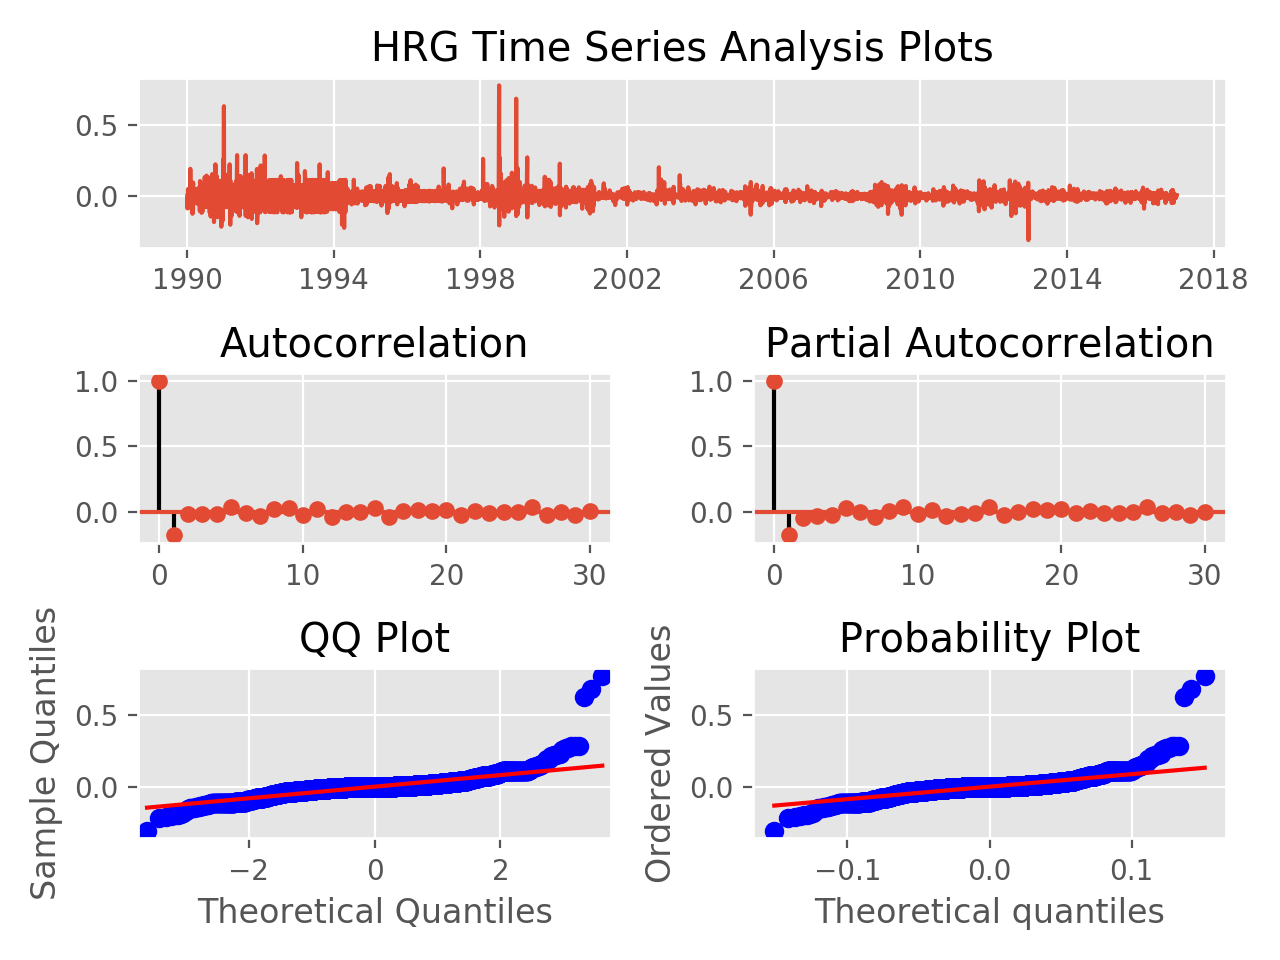
\includegraphics[width=\textwidth]{HRG-time-series.png}
    \captionof{figure}{HRG time series analysis}
    \label{fig:nonfloat}
\end{center}

\begin{center}  
    \includegraphics[width=\textwidth]{HRG-histogram.png}
    \captionof{figure}{HRG histogram of returns}
    \label{fig:nonfloat}
\end{center}

\begin{center}
    \includegraphics[width=\textwidth]{HL-time-series.png}
    \captionof{figure}{HL time series analysis}
    \label{fig:nonfloat}
\end{center}

\begin{center}  
    \includegraphics[width=\textwidth]{HL-histogram.png}
    \captionof{figure}{HL histogram of returns}
    \label{fig:nonfloat}
\end{center}

\subsection{Ordinary Least Squares (OLS)}
MSFT scored a mean absolute error regression loss of 0.810, and a coefficient of determination of 0.991.

\begin{center}
    \includegraphics[width=\textwidth]{MSFT-OLS-In-Sample-Prediction.png}
    \captionof{figure}{MSFT OLS in-sample prediction}
    \label{fig:nonfloat}
\end{center}

\begin{center}  
    \includegraphics[width=\textwidth]{100-Day-MSFT-OLS-Out-of-Sample-Forecast.png}
    \captionof{figure}{100 day MSFT OLS in-sample forecast}
    \label{fig:nonfloat}
\end{center}

CDE scored a mean absolute error regression loss of 0.985, and a coefficient of determination of 0.973.

\begin{center}
    \includegraphics[width=\textwidth]{CDE-OLS-In-Sample-Prediction.png}
    \captionof{figure}{CDE OLS in-sample prediction}
    \label{fig:nonfloat}
\end{center}

\begin{center}
    \includegraphics[width=\textwidth]{100-Day-CDE-OLS-Out-of-Sample-Forecast.png}
    \captionof{figure}{100 Day CDE OLS out of sample forecast}
    \label{fig:nonfloat}
\end{center}

NAVB scored a mean absolute error regression loss of 0.124, and a coefficient of determination of 0.966.

\begin{center}  
    \includegraphics[width=\textwidth]{NAVB-OLS-In-Sample-Prediction.png}
    \captionof{figure}{NAVB OLS in-sample prediction}
    \label{fig:nonfloat}
\end{center}

\begin{center}
  
    \includegraphics[width=\textwidth]{100-Day-NAVB-OLS-Out-of-Sample-Forecast.png}
    \captionof{figure}{100 day NAVB OLS in-sample forecast}
    \label{fig:nonfloat}
\end{center}

HRG scored a mean absolute error regression loss of 0.291, and a coefficient of determination of 0.986.

\begin{center}  
    \includegraphics[width=\textwidth]{HRG-OLS-In-Sample-Prediction.png}
    \captionof{figure}{HRG OLS in-sample prediction}
    \label{fig:nonfloat}
\end{center}

\begin{center}
    \includegraphics[width=\textwidth]{100-Day-HRG-OLS-Out-of-Sample-Forecast.png}
    \captionof{figure}{100 day HRG OLS in-sample forecast}
    \label{fig:nonfloat}
\end{center}

HL scored a mean absolute error regression loss of 0.336, and a coefficient of determination of 0.963.

\begin{center}  
    \includegraphics[width=\textwidth]{HL-OLS-In-Sample-Prediction.png}
    \captionof{figure}{HL OLS in-sample prediction}
    \label{fig:nonfloat}
\end{center}

\begin{center}
    \includegraphics[width=\textwidth]{100-Day-HL-OLS-Out-of-Sample-Forecast.png}
    \captionof{figure}{100 day HL OLS in-sample forecast}
    \label{fig:nonfloat}
\end{center}

\subsection{Auto Regressive (AR)}

MSFT scored sharpe ratios of 1.152 for the original returns, and -34.641 for the predicted returns in the in-sample test.

\begin{center}  
    \includegraphics[width=\textwidth]{MSFT-AR-time-series.png}
    \captionof{figure}{MSFT AR time series analysis}
    \label{fig:nonfloat}
\end{center}

\begin{center}
    \includegraphics[width=\textwidth]{MSFT-AR-histogram.png}
    \captionof{figure}{MSFT AR histogram of returns}
    \label{fig:nonfloat}
\end{center}

\begin{center}  
    \includegraphics[width=\textwidth]{MSFT-AR-In-Sample-Return-Prediction.png}
    \captionof{figure}{MSFT AR in-sample returns prediction}
    \label{fig:nonfloat}
\end{center}

\begin{center}
    \includegraphics[width=\textwidth]{100-Day-MSFT-AR-Out-of-Sample-Return-Forecast.png}
    \captionof{figure}{100 day MSFT AR in-sample returns forecast}
    \label{fig:nonfloat}
\end{center}

CDE scored sharpe ratios of -1.050 for the original returns, and -0.239 for the predicted returns in the in-sample test.

\begin{center}
    \includegraphics[width=\textwidth]{CDE-AR-time-series.png}
    \captionof{figure}{CDE AR time series analysis}
    \label{fig:nonfloat}
\end{center}

\begin{center}
    \includegraphics[width=\textwidth]{CDE-AR-histogram.png}
    \captionof{figure}{CDE AR histogram of returns}
    \label{fig:nonfloat}
\end{center}

\begin{center}
    \includegraphics[width=\textwidth]{CDE-AR-In-Sample-Return-Prediction.png}
    \captionof{figure}{CDE AR in-sample returns prediction}
    \label{fig:nonfloat}
\end{center}

\begin{center}
    \includegraphics[width=\textwidth]{100-Day-CDE-AR-Out-of-Sample-Return-Forecast.png}
    \captionof{figure}{100 day CDE AR in-sample returns forecast}
    \label{fig:nonfloat}
\end{center}

NAVB scored sharpe ratios of -0.410 for the original returns, and 0.124 for the predicted returns in the in-sample test.

\begin{center}
    \includegraphics[width=\textwidth]{NAVB-AR-time-series.png}
    \captionof{figure}{NAVB AR time series analysis}
    \label{fig:nonfloat}
\end{center}

\begin{center}
    \includegraphics[width=\textwidth]{NAVB-AR-histogram.png}
    \captionof{figure}{NAVB AR histogram of returns}
    \label{fig:nonfloat}
\end{center}

\begin{center}
    \includegraphics[width=\textwidth]{NAVB-AR-In-Sample-Return-Prediction.png}
    \captionof{figure}{NAVB AR in-sample returns prediction}
    \label{fig:nonfloat}
\end{center}

\begin{center}
    \includegraphics[width=\textwidth]{100-Day-NAVB-AR-Out-of-Sample-Return-Forecast.png}
    \captionof{figure}{100 day NAVB AR in-sample returns forecast}
    \label{fig:nonfloat}
\end{center}

HRG scored sharpe ratios of 0.627 for the original returns, and -2.603 for the predicted returns in the in-sample test.

\begin{center}  
    \includegraphics[width=\textwidth]{HRG-AR-time-series.png}
    \captionof{figure}{HRG AR time series analysis}
    \label{fig:nonfloat}
\end{center}

\begin{center}
  
    \includegraphics[width=\textwidth]{HRG-AR-histogram.png}
    \captionof{figure}{HRG AR histogram of returns}
    \label{fig:nonfloat}
\end{center}

\begin{center}
    \includegraphics[width=\textwidth]{HRG-AR-In-Sample-Return-Prediction.png}
    \captionof{figure}{HL AR in-sample returns prediction}
    \label{fig:nonfloat}
\end{center}

\begin{center}
    \includegraphics[width=\textwidth]{100-Day-HRG-AR-Out-of-Sample-Return-Forecast.png}
    \captionof{figure}{100 day HRG AR in-sample returns forecast}
    \label{fig:nonfloat}
\end{center}

HL scored sharpe ratios of 0.695 for the original returns, and -1.880 for the predicted returns in the in-sample test.

\begin{center}  
    \includegraphics[width=\textwidth]{HL-AR-time-series.png}
    \captionof{figure}{HL AR time series analysis}
    \label{fig:nonfloat}
\end{center}

\begin{center}
    \includegraphics[width=\textwidth]{HL-AR-histogram.png}
    \captionof{figure}{HL AR histogram of returns}
    \label{fig:nonfloat}
\end{center}

\begin{center}
  
    \includegraphics[width=\textwidth]{HL-AR-In-Sample-Return-Prediction.png}
    \captionof{figure}{HL AR in-sample returns prediction}
    \label{fig:nonfloat}
\end{center}

\begin{center}
  
    \includegraphics[width=\textwidth]{100-Day-HL-AR-Out-of-Sample-Return-Forecast.png}
    \captionof{figure}{100 day HL AR in-sample returns forecast}
    \label{fig:nonfloat}
\end{center}

\subsection{Moving Average (MA)}

MSFT scored sharpe ratios of 0.358 for the original returns, and -5.610 for the predicted returns in the in-sample test.

\begin{center}
    \includegraphics[width=\textwidth]{MSFT-MA-time-series.png}
  \captionof{figure}{MSFT MA time series analysis}
  \label{fig:nonfloat}
\end{center}

\begin{center}
    \includegraphics[width=\textwidth]{MSFT-MA-histogram.png}
    \captionof{figure}{MSFT MA histogram of returns}
    \label{fig:nonfloat}
\end{center}

\begin{center}  
    \includegraphics[width=\textwidth]{MSFT-MA-In-Sample-Return-Prediction.png}
    \captionof{figure}{MSFT MA in-sample returns prediction}
    \label{fig:nonfloat}
\end{center}

\begin{center}  
    \includegraphics[width=\textwidth]{100-Day-MSFT-MA-Out-of-Sample-Return-Forecast.png}
    \captionof{figure}{100 day MSFT MA in-sample returns forecast}
    \label{fig:nonfloat}
\end{center}

CDE scored sharpe ratios of -0.199 for the original returns, and -0.760 for the predicted returns in the in-sample test.

\begin{center}
    \includegraphics[width=\textwidth]{CDE-MA-time-series.png}
    \captionof{figure}{CDE MA time series analysis}
    \label{fig:nonfloat}
\end{center}

\begin{center}  
    \includegraphics[width=\textwidth]{CDE-MA-histogram.png}
    \captionof{figure}{CDE MA histogram of returns}
    \label{fig:nonfloat}
\end{center}

\begin{center}  
    \includegraphics[width=\textwidth]{CDE-MA-In-Sample-Return-Prediction.png}
    \captionof{figure}{CDE MA in-sample returns prediction}
    \label{fig:nonfloat}
\end{center}

\begin{center}
    \includegraphics[width=\textwidth]{100-Day-CDE-MA-Out-of-Sample-Return-Forecast.png}
    \captionof{figure}{100 day CDE MA in-sample returns forecast}
    \label{fig:nonfloat}
\end{center}

NAVB scored sharpe ratios of -0.067 for the original returns, and 0.590 for the predicted returns in the in-sample test.

\begin{center}  
    \includegraphics[width=\textwidth]{NAVB-MA-time-series.png}
    \captionof{figure}{NAVB MA time series analysis}
    \label{fig:nonfloat}
\end{center}

\begin{center}  
    \includegraphics[width=\textwidth]{NAVB-MA-histogram.png}
    \captionof{figure}{NAVB MA histogram of returns}
    \label{fig:nonfloat}
\end{center}

\begin{center}
    \includegraphics[width=\textwidth]{NAVB-MA-In-Sample-Return-Prediction.png}
    \captionof{figure}{NAVB MA in-sample returns prediction}
    \label{fig:nonfloat}
\end{center}

\begin{center}
    \includegraphics[width=\textwidth]{100-Day-NAVB-MA-Out-of-Sample-Return-Forecast.png}
    \captionof{figure}{100 day NAVB MA in-sample returns forecast}
    \label{fig:nonfloat}
\end{center}

HRG scored sharpe ratios of 0.084 for the original returns, and -1.020 for the predicted returns in the in-sample test.

\begin{center}  
    \includegraphics[width=\textwidth]{HRG-MA-time-series.png}
    \captionof{figure}{HRG MA time series analysis}
    \label{fig:nonfloat}
\end{center}

\begin{center}  
    \includegraphics[width=\textwidth]{HRG-MA-histogram.png}
    \captionof{figure}{HRG MA histogram of returns}
    \label{fig:nonfloat}
\end{center}

\begin{center}
    \includegraphics[width=\textwidth]{HRG-MA-In-Sample-Return-Prediction.png}
    \captionof{figure}{HRG MA in-sample returns prediction}
    \label{fig:nonfloat}
\end{center}

\begin{center}
    \includegraphics[width=\textwidth]{100-Day-HRG-MA-Out-of-Sample-Return-Forecast.png}
    \captionof{figure}{100 day HRG MA in-sample returns forecast}
    \label{fig:nonfloat}
\end{center}

HL scored sharpe ratios of -0.128 for the original returns, and -0.977 for the predicted returns in the in-sample test.

\begin{center}
    \includegraphics[width=\textwidth]{HL-MA-time-series.png}
    \captionof{figure}{HL MA time series analysis}
    \label{fig:nonfloat}
\end{center}

\begin{center}
    \includegraphics[width=\textwidth]{HL-MA-histogram.png}
    \captionof{figure}{HL MA histogram of returns}
    \label{fig:nonfloat}
\end{center}

\begin{center}
    \includegraphics[width=\textwidth]{HL-MA-In-Sample-Return-Prediction.png}
    \captionof{figure}{HL MA in-sample returns prediction}
    \label{fig:nonfloat}
\end{center}

\begin{center}
    \includegraphics[width=\textwidth]{100-Day-HL-MA-Out-of-Sample-Return-Forecast.png}
    \captionof{figure}{100 day HL MA in-sample returns forecast}
    \label{fig:nonfloat}
\end{center}

\subsection{Auto Regressive Moving Average (ARMA)}

HL scored sharpe ratios of 0.537 for the original returns, and -6.485 for the predicted returns in the in-sample test.

\begin{center}  
    \includegraphics[width=\textwidth]{MSFT-ARMA-time-series.png}
    \captionof{figure}{MSFT ARMA time series analysis}
    \label{fig:nonfloat}
\end{center}

\begin{center}
    \includegraphics[width=\textwidth]{MSFT-ARMA-histogram.png}
    \captionof{figure}{MSFT ARMA histogram of returns}
    \label{fig:nonfloat}
\end{center}

\begin{center}
    \includegraphics[width=\textwidth]{MSFT-ARMA-In-Sample-Return-Prediction.png}
    \captionof{figure}{MSFT ARMA in-sample returns prediction}
    \label{fig:nonfloat}
\end{center}

\begin{center}
    \includegraphics[width=\textwidth]{100-Day-MSFT-ARMA-Out-of-Sample-Return-Forecast.png}
    \captionof{figure}{100 day MSFT ARMA in-sample returns forecast}
    \label{fig:nonfloat}
\end{center}

MSFT scored sharpe ratios of -0.128 for the original returns, and -0.977 for the predicted returns in the in-sample test.

\begin{center}
    \includegraphics[width=\textwidth]{CDE-ARMA-time-series.png}
    \captionof{figure}{CDE ARMA time series analysis}
    \label{fig:nonfloat}
\end{center}

\begin{center}
    \includegraphics[width=\textwidth]{CDE-ARMA-histogram.png}
    \captionof{figure}{CDE ARMA histogram of returns}
    \label{fig:nonfloat}
\end{center}

\begin{center}
    \includegraphics[width=\textwidth]{CDE-ARMA-In-Sample-Return-Prediction.png}
    \captionof{figure}{CDE ARMA in-sample returns prediction}
    \label{fig:nonfloat}
\end{center}

\begin{center}
    \includegraphics[width=\textwidth]{100-Day-CDE-ARMA-Out-of-Sample-Return-Forecast.png}
    \captionof{figure}{100 day CDE ARMA in-sample returns forecast}
    \label{fig:nonfloat}
\end{center}

CDE scored sharpe ratios of -0.245 for the original returns, and -0.614 for the predicted returns in the in-sample test.

\begin{center}  
    \includegraphics[width=\textwidth]{NAVB-ARMA-time-series.png}
    \captionof{figure}{NAVB ARMA time series analysis}
    \label{fig:nonfloat}
\end{center}

\begin{center}
    \includegraphics[width=\textwidth]{NAVB-ARMA-histogram.png}
    \captionof{figure}{NAVB ARMA histogram of returns}
    \label{fig:nonfloat}
\end{center}

\begin{center}  
    \includegraphics[width=\textwidth]{NAVB-ARMA-In-Sample-Return-Prediction.png}
    \captionof{figure}{NAVB ARMA in-sample returns prediction}
    \label{fig:nonfloat}
\end{center}

\begin{center}  
    \includegraphics[width=\textwidth]{100-Day-NAVB-ARMA-Out-of-Sample-Return-Forecast.png}
    \captionof{figure}{100 day NAVB ARMA in-sample returns forecast}
    \label{fig:nonfloat}
\end{center}

NAVB scored sharpe ratios of -0.032 for the original returns, and -0.641 for the predicted returns in the in-sample test.

\begin{center}
    \includegraphics[width=\textwidth]{HRG-ARMA-time-series.png}
    \captionof{figure}{HRG ARMA time series analysis}
    \label{fig:nonfloat}
\end{center}

\begin{center}
    \includegraphics[width=\textwidth]{HRG-ARMA-histogram.png}
    \captionof{figure}{HRG ARMA histogram of returns}
    \label{fig:nonfloat}
\end{center}

\begin{center}
    \includegraphics[width=\textwidth]{HRG-ARMA-In-Sample-Return-Prediction.png}
    \captionof{figure}{HRG ARMA in-sample returns prediction}
    \label{fig:nonfloat}
\end{center}

\begin{center}
    \includegraphics[width=\textwidth]{100-Day-HRG-ARMA-Out-of-Sample-Return-Forecast.png}
    \captionof{figure}{100 day HRG ARMA in-sample returns forecast}
    \label{fig:nonfloat}
\end{center}

HL scored sharpe ratios of 0.111 for the original returns, and -1.023 for the predicted returns in the in-sample test.

\begin{center}
  
    \includegraphics[width=\textwidth]{HL-ARMA-time-series.png}
    \captionof{figure}{HL ARMA time series analysis}
    \label{fig:nonfloat}
\end{center}

\begin{center}  
    \includegraphics[width=\textwidth]{HL-ARMA-histogram.png}
    \captionof{figure}{HL ARMA histogram of returns}
    \label{fig:nonfloat}
\end{center}

\begin{center}
    \includegraphics[width=\textwidth]{HL-ARMA-In-Sample-Return-Prediction.png}
    \captionof{figure}{HL ARMA in-sample returns prediction}
    \label{fig:nonfloat}
\end{center}

\begin{center}
    \includegraphics[width=\textwidth]{100-Day-HL-ARMA-Out-of-Sample-Return-Forecast.png}
    \captionof{figure}{100 day HL ARMA in-sample returns forecast}
    \label{fig:nonfloat}
\end{center}

\subsection{Auto Regressive Integrated Moving Average (ARIMA)}

MSFT scored sharpe ratios of 0.123 for the original returns, and -4.904 for the predicted returns in the in-sample test.

\begin{center}  
    \includegraphics[width=\textwidth]{MSFT-ARIMA-time-series.png}
    \captionof{figure}{MSFT ARIMA time series analysis}
    \label{fig:nonfloat}
\end{center}

\begin{center}
    \includegraphics[width=\textwidth]{MSFT-ARIMA-histogram.png}
    \captionof{figure}{MSFT ARIMA histogram of returns}
    \label{fig:nonfloat}
\end{center}

\begin{center}  
    \includegraphics[width=\textwidth]{MSFT-ARIMA-In-Sample-Return-Prediction.png}
    \captionof{figure}{MSFT ARIMA in-sample returns prediction}
    \label{fig:nonfloat}
\end{center}

\begin{center}
    \includegraphics[width=\textwidth]{100-Day-MSFT-ARIMA-Out-of-Sample-Return-Forecast.png}
    \captionof{figure}{100 day MSFT ARIMA in-sample returns forecast}
    \label{fig:nonfloat}
\end{center}

CDE scored sharpe ratios of -0.133 for the original returns, and -0.698 for the predicted returns in the in-sample test.

\begin{center}
    \includegraphics[width=\textwidth]{CDE-ARIMA-time-series.png}
    \captionof{figure}{CDE ARIMA time series analysis}
    \label{fig:nonfloat}
\end{center}

\begin{center}
    \includegraphics[width=\textwidth]{CDE-ARIMA-histogram.png}
    \captionof{figure}{CDE ARIMA histogram of returns}
    \label{fig:nonfloat}
\end{center}

\begin{center}  
    \includegraphics[width=\textwidth]{CDE-ARIMA-In-Sample-Return-Prediction.png}
    \captionof{figure}{CDE ARIMA in-sample returns prediction}
    \label{fig:nonfloat}
\end{center}

\begin{center}
    \includegraphics[width=\textwidth]{100-Day-CDE-ARIMA-Out-of-Sample-Return-Forecast.png}
    \captionof{figure}{100 day CDE ARIMA in-sample returns forecast}
    \label{fig:nonfloat}
\end{center}

NAVB scored sharpe ratios of 0.015 for the original returns, and -0.708 for the predicted returns in the in-sample test.

\begin{center}  
    \includegraphics[width=\textwidth]{NAVB-ARIMA-time-series.png}
    \captionof{figure}{NAVB ARIMA time series analysis}
    \label{fig:nonfloat}
\end{center}

\begin{center}
    \includegraphics[width=\textwidth]{NAVB-ARIMA-histogram.png}
    \captionof{figure}{NAVB ARIMA histogram of returns}
    \label{fig:nonfloat}
\end{center}

\begin{center}  
    \includegraphics[width=\textwidth]{NAVB-ARIMA-In-Sample-Return-Prediction.png}
    \captionof{figure}{NAVB ARIMA in-sample returns prediction}
    \label{fig:nonfloat}
\end{center}

\begin{center}
    \includegraphics[width=\textwidth]{100-Day-NAVB-ARIMA-Out-of-Sample-Return-Forecast.png}
    \captionof{figure}{100 day NAVB ARIMA in-sample returns forecast}
    \label{fig:nonfloat}
\end{center}

HRG scored sharpe ratios of 0.401 for the original returns, and -1.354 for the predicted returns in the in-sample test.

\begin{center}
    \includegraphics[width=\textwidth]{HRG-ARIMA-time-series.png}
    \captionof{figure}{HRG ARIMA time series analysis}
    \label{fig:nonfloat}
\end{center}

\begin{center}
    \includegraphics[width=\textwidth]{HRG-ARIMA-histogram.png}
    \captionof{figure}{HRG ARIMA histogram of returns}
    \label{fig:nonfloat}
\end{center}

\begin{center}
    \includegraphics[width=\textwidth]{HRG-ARIMA-In-Sample-Return-Prediction.png}
    \captionof{figure}{HRG ARIMA in-sample returns prediction}
    \label{fig:nonfloat}
\end{center}

\begin{center}
    \includegraphics[width=\textwidth]{100-Day-HRG-ARIMA-Out-of-Sample-Return-Forecast.png}
    \captionof{figure}{100 day HRG ARIMA in-sample returns forecast}
    \label{fig:nonfloat}
\end{center}

HL scored sharpe ratios of -0.127 for the original returns, and -0.974 for the predicted returns in the in-sample test.

\begin{center}
    \includegraphics[width=\textwidth]{HL-ARIMA-time-series.png}
    \captionof{figure}{HL ARIMA time series analysis}
    \label{fig:nonfloat}
\end{center}

\begin{center}
    \includegraphics[width=\textwidth]{HL-ARIMA-histogram.png}
    \captionof{figure}{HL ARIMA histogram of returns}
    \label{fig:nonfloat}
\end{center}

\begin{center}
    \includegraphics[width=\textwidth]{HL-ARIMA-In-Sample-Return-Prediction.png}
    \captionof{figure}{HL ARIMA in-sample returns prediction}
    \label{fig:nonfloat}
\end{center}

\begin{center}  
    \includegraphics[width=\textwidth]{100-Day-HL-ARIMA-Out-of-Sample-Return-Forecast.png}
    \captionof{figure}{100 day HL ARIMA in-sample returns forecast}
    \label{fig:nonfloat}
\end{center}

\section{Machine Learning}

\subsection{Classification}

\subsubsection{Decision Tree}

\begin{center}
    \begin{tabular}{ | l | l | l | | l | l | l | p{5cm} |}
    \hline
    Ticker & Precision & True Negatives & False Negatives & True Positives & False Positives \\ \hline
    MSFT & 0.77 & 493 & 131 & 547 & 190 \\ \hline
    CDE & 0.79 & 565 & 144 & 504 & 133 \\ \hline
    NAVB & 0.76 & 592 & 165 & 331 & 126 \\ \hline
    HRG & 0.75 & 553 & 210 & 462 & 135 \\ \hline
    HL & 0.79 & 603 & 135 & 475 & 147 \\
    \hline
    \end{tabular}
    \captionof{table}{Decision Tree results}
    \label{table:nonfloat}
\end{center}

\subsubsection{Boosted Decision Tree}

\begin{center}
    \begin{tabular}{ | l | l | l | | l | l | l | p{5cm} |}
    \hline
    Ticker & Precision & True Negatives & False Negatives & True Positives & False Positives \\ \hline
    MSFT & 0.77 & 493 & 130 & 548 & 190 \\ \hline
    CDE & 0.79 & 564 & 143 & 505 & 134 \\ \hline
    NAVB & 0.76 & 588 & 164 & 332 & 130 \\ \hline
    HRG & 0.75 & 542 & 191 & 481 & 146 \\ \hline
    HL & 0.79 & 602 & 132 & 478 & 149 \\
    \hline
    \end{tabular}
    \captionof{table}{Boosted Decision Tree results}
    \label{table:nonfloat}
\end{center}

\subsubsection{Support Vector Machine (SVM)}

\begin{center}
    \begin{tabular}{ | l | l | l | | l | l | l | p{5cm} |}
    \hline
    Ticker & Precision & True Negatives & False Negatives & True Positives & False Positives \\ \hline
    MSFT & 0.77 & 493 & 130 & 548 & 190 \\ \hline
    CDE & 0.79 & 564 & 143 & 505 & 134 \\ \hline
    NAVB & 0.76 & 593 & 169 & 327 & 125 \\ \hline
    HRG & 0.75 & 542 & 191 & 481 & 146 \\ \hline
    HL & 0.81 & 579 & 98 & 512 & 171 \\
    \hline
    \end{tabular}
    \captionof{table}{Support Vector Machine results}
    \label{table:nonfloat}
\end{center}

\subsubsection{Random Forest}

\begin{center}    
    \begin{tabular}{ | l | l | l | | l | l | l | p{5cm} |}
    \hline
    Ticker & Precision & True Negatives & False Negatives & True Positives & False Positives \\ \hline
    MSFT & 0.77 & 493 & 131 & 547 & 190 \\ \hline
    CDE & 0.79 & 566 & 145 & 503 & 132 \\ \hline
    NAVB & 0.76 & 590 & 164 & 332 & 128 \\ \hline
    HRG & 0.75 & 554 & 210 & 462 & 134 \\ \hline
    HL & 0.81 & 581 & 101 & 509 & 169 \\
    \hline
    \end{tabular}
    \captionof{table}{Random Forest results}
    \label{table:nonfloat}
\end{center}

\subsubsection{K-Nearest Neighbour}

\begin{center}
    \begin{tabular}{ | l | l | l | | l | l | l | p{5cm} |}
    \hline
    Ticker & Precision & True Negatives & False Negatives & True Positives & False Positives \\ \hline
    MSFT & 0.76 & 489 & 130 & 548 & 194 \\ \hline
    CDE & 0.80 & 574 & 147 & 501 & 126 \\ \hline
    NAVB & 0.75 & 573 & 161 & 335 & 145 \\ \hline
    HRG & 0.74 & 560 & 233 & 439 & 128 \\ \hline
    HL & 0.81 & 581 & 101 & 509 & 169 \\
    \hline
    \end{tabular}
    \captionof{table}{K-Nearest Neighbour results}
    \label{table:nonfloat}
\end{center}

\subsubsection{Logistic Regression}

\begin{center}
    \begin{tabular}{ | l | l | l | | l | l | l | p{5cm} |}
    \hline
    Ticker & Precision & True Negatives & False Negatives & True Positives & False Positives \\ \hline
    MSFT & 0.77 & 493 & 130 & 548 & 190 \\ \hline
    CDE & 0.79 & 564 & 143 & 505 & 134 \\ \hline
    NAVB & 0.76 & 588 & 164 & 332 & 130 \\ \hline
    HRG & 0.75 & 542 & 191 & 481 & 146 \\ \hline
    HL & 0.79 & 601 & 132 & 478 & 149 \\
    \hline
    \end{tabular}
    \captionof{table}{Logistic Regression results}
    \label{table:nonfloat}
\end{center}

\subsubsection{Gaussian Naive Bayes}

\begin{center}
    \begin{tabular}{ | l | l | l | | l | l | l | p{5cm} |}
    \hline
    Ticker & Precision & True Negatives & False Negatives & True Positives & False Positives \\ \hline
    MSFT & 0.73 & 478 & 168 & 510 & 205 \\ \hline
    CDE & 0.76 & 555 & 187 & 461 & 143 \\ \hline
    NAVB & 0.74 & 553 & 153 & 343 & 165 \\ \hline
    HRG & 0.73 & 491 & 170 & 502 & 197 \\ \hline
    HL & 0.77 & 590 & 157 & 453 & 160 \\
    \hline
    \end{tabular}
    \captionof{table}{Gaussian Naive Bayes results}
    \label{table:nonfloat}
\end{center}

\subsubsection{Bernoulli Naive Bayes}

\begin{center}
    \begin{tabular}{ | l | l | l | | l | l | l | p{5cm} |}
    \hline
    Ticker & Precision & True Negatives & False Negatives & True Positives & False Positives \\ \hline
    MSFT & 0.73 & 479 & 169 & 509 & 204 \\ \hline
    CDE & 0.76 & 558 & 187 & 461 & 140 \\ \hline
    NAVB & 0.74 & 553 & 153 & 343 & 165 \\ \hline
    HRG & 0.73 & 492 & 170 & 502 & 196 \\ \hline
    HL & 0.77 & 590 & 158 & 452 & 160 \\
    \hline
    \end{tabular}
    \captionof{table}{Bernoulli Naive Bayes results}
    \label{table:nonfloat}
\end{center}

\subsubsection{Neural Network}

\begin{center}
    \begin{tabular}{ | l | l | l | | l | l | l | p{5cm} |}
    \hline
    Ticker & Precision & True Negatives & False Negatives & True Positives & False Positives \\ \hline
    MSFT & 0.77 & 685 & 181 & 787 & 258 \\ \hline
    CDE & 0.79 & 616 & 156 & 542 & 152 \\ \hline
    NAVB & 0.76 & 691 & 183 & 403 & 153 \\ \hline
    HRG & 0.74 & 690 & 269 & 542 & 164 \\ \hline
    HL & 0.77 & 1059 & 270 & 848 & 164 \\
    \hline
    \end{tabular}
    \captionof{table}{Neural Network results}
    \label{table:nonfloat}
\end{center}

\subsubsection{Stochastic Gradient Descent}

\begin{center}
    \begin{tabular}{ | l | l | l | | l | l | l | p{5cm} |}
    \hline
    Ticker & Precision & True Negatives & False Negatives & True Positives & False Positives \\ \hline
    MSFT & 0.77 & 493 & 130 & 548 & 190 \\ \hline
    CDE & 0.76 & 462 & 106 & 542 & 236 \\ \hline
    NAVB & 0.59 & 1032 & 707 & 118 & 80 \\ \hline
    HRG & 0.72 & 761 & 225 & 1059 & 518 \\ \hline
    HL & 0.80 & 535 & 83 & 527 & 215 \\
    \hline
    \end{tabular}
    \captionof{table}{Stochastic Gradient Descent results}
    \label{table:nonfloat}
\end{center}

\subsection{Regression}

\subsubsection{Decision Tree}
MSFT scored a mean absolute error regression loss of 5.606, and a coefficient of determination of 0.458.

\begin{center}
    \includegraphics[width=\textwidth]{MSFT-Decision-Trees-In-Sample-Prediction.png}
    \captionof{figure}{MSFT Decision Trees in-sample prediction}
    \label{fig:nonfloat}
\end{center}

\begin{center}  
    \includegraphics[width=\textwidth]{100-Day-MSFT-Decision-Trees-Out-of-Sample-Forecast.png}
    \captionof{figure}{100 day MSFT Decision Trees out-of-sample forecast}
    \label{fig:nonfloat}
\end{center}

CDE scored a mean absolute error regression loss of 2.906, and a coefficient of determination of 0.816.

\begin{center}
    \includegraphics[width=\textwidth]{CDE-Decision-Trees-In-Sample-Prediction.png}
    \captionof{figure}{CDE Decision Trees in-sample prediction}
    \label{fig:nonfloat}
\end{center}

\begin{center}  
    \includegraphics[width=\textwidth]{100-Day-CDE-Decision-Trees-Out-of-Sample-Forecast.png}
    \captionof{figure}{100 day CDE Decision Trees out-of-sample forecast}
    \label{fig:nonfloat}
\end{center}

NAVB scored a mean absolute error regression loss of 0.422, and a coefficient of determination of 0.693.

\begin{center}
    \includegraphics[width=\textwidth]{NAVB-Decision-Trees-In-Sample-Prediction.png}
    \captionof{figure}{NAVB Decision Trees in-sample prediction}
    \label{fig:nonfloat}
\end{center}

\begin{center}  
    \includegraphics[width=\textwidth]{100-Day-NAVB-Decision-Trees-Out-of-Sample-Forecast.png}
    \captionof{figure}{100 day NAVB Decision Trees out-of-sample forecast}
    \label{fig:nonfloat}
\end{center}

HRG scored a mean absolute error regression loss of 1.415, and a coefficient of determination of 0.464.

\begin{center}
    \includegraphics[width=\textwidth]{HRG-Decision-Trees-In-Sample-Prediction.png}
    \captionof{figure}{HRG Decision Trees in-sample prediction}
    \label{fig:nonfloat}
\end{center}

\begin{center}  
    \includegraphics[width=\textwidth]{100-Day-HRG-Decision-Trees-Out-of-Sample-Forecast.png}
    \captionof{figure}{100 day HRG Decision Trees out-of-sample forecast}
    \label{fig:nonfloat}
\end{center}

HL scored a mean absolute error regression loss of 0.506, and a coefficient of determination of 0.923.

\begin{center}
    \includegraphics[width=\textwidth]{HL-Decision-Trees-In-Sample-Prediction.png}
    \captionof{figure}{HL Decision Trees in-sample prediction}
    \label{fig:nonfloat}
\end{center}

\begin{center}  
    \includegraphics[width=\textwidth]{100-Day-HL-Decision-Trees-Out-of-Sample-Forecast.png}
    \captionof{figure}{100 day HL Decision Trees out-of-sample forecast}
    \label{fig:nonfloat}
\end{center}

\subsubsection{Boosted Decision Tree}
MSFT scored a mean absolute error regression loss of 4.426, and a coefficient of determination of 0.580.

\begin{center}
    \includegraphics[width=\textwidth]{MSFT-Boosted-Trees-In-Sample-Prediction.png}
    \captionof{figure}{MSFT Boosted Decision Trees in-sample prediction}
    \label{fig:nonfloat}
\end{center}

\begin{center}  
    \includegraphics[width=\textwidth]{100-Day-MSFT-Boosted-Trees-Out-of-Sample-Forecast.png}
    \captionof{figure}{100 day MSFT Boosted Decision Trees out-of-sample forecast}
    \label{fig:nonfloat}
\end{center}

CDE scored a mean absolute error regression loss of 5.452, and a coefficient of determination of 0.581.

\begin{center}
    \includegraphics[width=\textwidth]{CDE-Boosted-Trees-In-Sample-Prediction.png}
    \captionof{figure}{CDE Boosted Decision Trees in-sample prediction}
    \label{fig:nonfloat}
\end{center}

\begin{center}  
    \includegraphics[width=\textwidth]{100-Day-CDE-Boosted-Trees-Out-of-Sample-Forecast.png}
    \captionof{figure}{100 day CDE Boosted Decision Trees out-of-sample forecast}
    \label{fig:nonfloat}
\end{center}

NAVB scored a mean absolute error regression loss of 0.579, and a coefficient of determination of 0.509.

\begin{center}
    \includegraphics[width=\textwidth]{NAVB-Boosted-Trees-In-Sample-Prediction.png}
    \captionof{figure}{NAVB Boosted Decision Trees in-sample prediction}
    \label{fig:nonfloat}
\end{center}

\begin{center}  
    \includegraphics[width=\textwidth]{100-Day-NAVB-Boosted-Trees-Out-of-Sample-Forecast.png}
    \captionof{figure}{100 day NAVB Boosted Decision Trees out-of-sample forecast}
    \label{fig:nonfloat}
\end{center}

HRG scored a mean absolute error regression loss of 0.980, and a coefficient of determination of 0.855.

\begin{center}
    \includegraphics[width=\textwidth]{HRG-Boosted-Trees-In-Sample-Prediction.png}
    \captionof{figure}{HRG Boosted Decision Trees in-sample prediction}
    \label{fig:nonfloat}
\end{center}

\begin{center}  
    \includegraphics[width=\textwidth]{100-Day-HRG-Boosted-Trees-Out-of-Sample-Forecast.png}
    \captionof{figure}{100 day HRG Boosted Decision Trees out-of-sample forecast}
    \label{fig:nonfloat}
\end{center}

HL scored a mean absolute error regression loss of 0.410, and a coefficient of determination of 0.952.

\begin{center}
    \includegraphics[width=\textwidth]{HL-Boosted-Trees-In-Sample-Prediction.png}
    \captionof{figure}{HL Boosted Decision Trees in-sample prediction}
    \label{fig:nonfloat}
\end{center}

\begin{center}  
    \includegraphics[width=\textwidth]{100-Day-HL-Boosted-Trees-Out-of-Sample-Forecast.png}
    \captionof{figure}{100 day HL Boosted Decision Trees out-of-sample forecast}
    \label{fig:nonfloat}
\end{center}

\subsubsection{K-Nearest Neighbour}
MSFT scored a mean absolute error regression loss of 4.426, and a coefficient of determination of 0.580.

\begin{center}
    \includegraphics[width=\textwidth]{MSFT-K-Nearest-Neighbour-In-Sample-Prediction.png}
    \captionof{figure}{MSFT K-Nearest Neighbour in-sample prediction}
    \label{fig:nonfloat}
\end{center}

\begin{center}  
    \includegraphics[width=\textwidth]{100-Day-MSFT-K-Nearest-Neighbour-Out-of-Sample-Forecast.png}
    \captionof{figure}{100 day MSFT K-Nearest Neighbour out-of-sample forecast}
    \label{fig:nonfloat}
\end{center}

CDE scored a mean absolute error regression loss of 5.452, and a coefficient of determination of 0.581.

\begin{center}
    \includegraphics[width=\textwidth]{CDE-K-Nearest-Neighbour-In-Sample-Prediction.png}
    \captionof{figure}{CDE K-Nearest Neighbour in-sample prediction}
    \label{fig:nonfloat}
\end{center}

\begin{center}  
    \includegraphics[width=\textwidth]{100-Day-CDE-K-Nearest-Neighbour-Out-of-Sample-Forecast.png}
    \captionof{figure}{100 day CDE K-Nearest Neighbour out-of-sample forecast}
    \label{fig:nonfloat}
\end{center}

NAVB scored a mean absolute error regression loss of 0.579, and a coefficient of determination of 0.509.

\begin{center}
    \includegraphics[width=\textwidth]{NAVB-K-Nearest-Neighbour-In-Sample-Prediction.png}
    \captionof{figure}{NAVB K-Nearest Neighbour in-sample prediction}
    \label{fig:nonfloat}
\end{center}

\begin{center}  
    \includegraphics[width=\textwidth]{100-Day-NAVB-K-Nearest-Neighbour-Out-of-Sample-Forecast.png}
    \captionof{figure}{100 day NAVB K-Nearest Neighbour out-of-sample forecast}
    \label{fig:nonfloat}
\end{center}

HRG scored a mean absolute error regression loss of 0.980, and a coefficient of determination of 0.855.

\begin{center}
    \includegraphics[width=\textwidth]{HRG-K-Nearest-Neighbour-In-Sample-Prediction.png}
    \captionof{figure}{HRG K-Nearest Neighbour in-sample prediction}
    \label{fig:nonfloat}
\end{center}

\begin{center}  
    \includegraphics[width=\textwidth]{100-Day-HRG-K-Nearest-Neighbour-Out-of-Sample-Forecast.png}
    \captionof{figure}{100 day HRG K-Nearest Neighbour out-of-sample forecast}
    \label{fig:nonfloat}
\end{center}

HL scored a mean absolute error regression loss of 0.410, and a coefficient of determination of 0.952.

\begin{center}
    \includegraphics[width=\textwidth]{HL-K-Nearest-Neighbour-In-Sample-Prediction.png}
    \captionof{figure}{HL K-Nearest Neighbour in-sample prediction}
    \label{fig:nonfloat}
\end{center}

\begin{center}  
    \includegraphics[width=\textwidth]{100-Day-HL-K-Nearest-Neighbour-Out-of-Sample-Forecast.png}
    \captionof{figure}{100 day HL K-Nearest Neighbour out-of-sample forecast}
    \label{fig:nonfloat}
\end{center}

\subsubsection{Random Forest}
MSFT scored a mean absolute error regression loss of 5.199, and a coefficient of determination of 0.483.

\begin{center}
    \includegraphics[width=\textwidth]{MSFT-Random-Forest-In-Sample-Prediction.png}
    \captionof{figure}{MSFT Random Forest in-sample prediction}
    \label{fig:nonfloat}
\end{center}

\begin{center}  
    \includegraphics[width=\textwidth]{100-Day-MSFT-Random-Forest-Out-of-Sample-Forecast.png}
    \captionof{figure}{100 day MSFT Random Forest out-of-sample forecast}
    \label{fig:nonfloat}
\end{center}

CDE scored a mean absolute error regression loss of 2.505, and a coefficient of determination of 0.861.

\begin{center}
    \includegraphics[width=\textwidth]{CDE-Random-Forest-In-Sample-Prediction.png}
    \captionof{figure}{CDE Random Forest in-sample prediction}
    \label{fig:nonfloat}
\end{center}

\begin{center}  
    \includegraphics[width=\textwidth]{100-Day-CDE-Random-Forest-Out-of-Sample-Forecast.png}
    \captionof{figure}{100 day CDE Random Forest out-of-sample forecast}
    \label{fig:nonfloat}
\end{center}

NAVB scored a mean absolute error regression loss of 0.293, and a coefficient of determination of 0.856.

\begin{center}
    \includegraphics[width=\textwidth]{NAVB-Random-Forest-In-Sample-Prediction.png}
    \captionof{figure}{NAVB Random Forest in-sample prediction}
    \label{fig:nonfloat}
\end{center}

\begin{center}  
    \includegraphics[width=\textwidth]{100-Day-NAVB-Random-Forest-Out-of-Sample-Forecast.png}
    \captionof{figure}{100 day NAVB Random Forest out-of-sample forecast}
    \label{fig:nonfloat}
\end{center}

HRG scored a mean absolute error regression loss of 0.675, and a coefficient of determination of 0.907.

\begin{center}
    \includegraphics[width=\textwidth]{HRG-Random-Forest-In-Sample-Prediction.png}
    \captionof{figure}{HRG Random Forest in-sample prediction}
    \label{fig:nonfloat}
\end{center}

\begin{center}  
    \includegraphics[width=\textwidth]{100-Day-HRG-Random-Forest-Out-of-Sample-Forecast.png}
    \captionof{figure}{100 day HRG Random Forest out-of-sample forecast}
    \label{fig:nonfloat}
\end{center}

HL scored a mean absolute error regression loss of 0.434, and a coefficient of determination of 0.922.

\begin{center}
    \includegraphics[width=\textwidth]{HL-Random-Forest-In-Sample-Prediction.png}
    \captionof{figure}{HL Random Forest in-sample prediction}
    \label{fig:nonfloat}
\end{center}

\begin{center}  
    \includegraphics[width=\textwidth]{100-Day-HL-Random-Forest-Out-of-Sample-Forecast.png}
    \captionof{figure}{100 day HL Random Forest out-of-sample forecast}
    \label{fig:nonfloat}
\end{center}

\subsubsection{Linear Regression}
MSFT scored a mean absolute error regression loss of 0.844, and a coefficient of determination of 0.990.

\begin{center}
    \includegraphics[width=\textwidth]{MSFT-Linear-Regression-In-Sample-Prediction.png}
    \captionof{figure}{MSFT Linear Regression in-sample prediction}
    \label{fig:nonfloat}
\end{center}

\begin{center}  
    \includegraphics[width=\textwidth]{100-Day-MSFT-Linear-Regression-Out-of-Sample-Forecast.png}
    \captionof{figure}{100 day MSFT Linear Regression out-of-sample forecast}
    \label{fig:nonfloat}
\end{center}

CDE scored a mean absolute error regression loss of 0.990, and a coefficient of determination of 0.972.

\begin{center}
    \includegraphics[width=\textwidth]{CDE-Linear-Regression-In-Sample-Prediction.png}
    \captionof{figure}{CDE Linear Regression in-sample prediction}
    \label{fig:nonfloat}
\end{center}

\begin{center}  
    \includegraphics[width=\textwidth]{100-Day-CDE-Linear-Regression-Out-of-Sample-Forecast.png}
    \captionof{figure}{100 day CDE Linear Regression out-of-sample forecast}
    \label{fig:nonfloat}
\end{center}

NAVB scored a mean absolute error regression loss of 0.128, and a coefficient of determination of 0.962.

\includegraphics[width=\textwidth]{NAVB-Linear-Regression-In-Sample-Prediction.png}

\includegraphics[width=\textwidth]{100-Day-NAVB-Linear-Regression-Out-of-Sample-Forecast.png}

\begin{center}
    \includegraphics[width=\textwidth]{CDE-Linear-Regression-In-Sample-Prediction.png}
    \captionof{figure}{CDE Linear Regression in-sample prediction}
    \label{fig:nonfloat}
\end{center}

\begin{center}  
    \includegraphics[width=\textwidth]{100-Day-CDE-Linear-Regression-Out-of-Sample-Forecast.png}
    \captionof{figure}{100 day CDE Linear Regression out-of-sample forecast}
    \label{fig:nonfloat}
\end{center}

HRG scored a mean absolute error regression loss of 0.324, and a coefficient of determination of 0.984.

\begin{center}
    \includegraphics[width=\textwidth]{HRG-Linear-Regression-In-Sample-Prediction.png}
    \captionof{figure}{HRG Linear Regression in-sample prediction}
    \label{fig:nonfloat}
\end{center}

\begin{center}  
    \includegraphics[width=\textwidth]{100-Day-HRG-Linear-Regression-Out-of-Sample-Forecast.png}
    \captionof{figure}{100 day HRG Linear Regression out-of-sample forecast}
    \label{fig:nonfloat}
\end{center}

HL scored a mean absolute error regression loss of 0.243, and a coefficient of determination of 0.964.

\begin{center}
    \includegraphics[width=\textwidth]{HL-Linear-Regression-In-Sample-Prediction.png}
    \captionof{figure}{HL Linear Regression in-sample prediction}
    \label{fig:nonfloat}
\end{center}

\begin{center}  
    \includegraphics[width=\textwidth]{100-Day-HL-Linear-Regression-Out-of-Sample-Forecast.png}
    \captionof{figure}{100 day HL Linear Regression out-of-sample forecast}
    \label{fig:nonfloat}
\end{center}

\subsubsection{Neural Network}
MSFT scored a mean absolute error regression loss of 1.073, and a coefficient of determination of 0.992.

\begin{center}
    \includegraphics[width=\textwidth]{MSFT-Neural-Network-In-Sample-Prediction.png}
    \captionof{figure}{MSFT Neural Network in-sample prediction}
    \label{fig:nonfloat}
\end{center}

\begin{center}  
    \includegraphics[width=\textwidth]{100-Day-MSFT-Neural-Network-Out-of-Sample-Forecast.png}
    \captionof{figure}{100 day MSFT Neural Network out-of-sample forecast}
    \label{fig:nonfloat}
\end{center}

CDE scored a mean absolute error regression loss of 2.906, and a coefficient of determination of 0.816.

\includegraphics[width=\textwidth]{CDE-Neural-Network-In-Sample-Prediction.png}

\includegraphics[width=\textwidth]{100-Day-CDE-Neural-Network-Out-of-Sample-Forecast.png}

\begin{center}
    \includegraphics[width=\textwidth]{CDE-Neural-Network-In-Sample-Prediction.png}
    \captionof{figure}{CDE Neural Network in-sample prediction}
    \label{fig:nonfloat}
\end{center}

\begin{center}  
    \includegraphics[width=\textwidth]{100-Day-CDE-Neural-Network-Out-of-Sample-Forecast.png}
    \captionof{figure}{100 day CDE Neural Network out-of-sample forecast}
    \label{fig:nonfloat}
\end{center}

NAVB scored a mean absolute error regression loss of 0.422, and a coefficient of determination of 0.693.

\begin{center}
    \includegraphics[width=\textwidth]{NAVB-Neural-Network-In-Sample-Prediction.png}
    \captionof{figure}{NAVB Neural Network in-sample prediction}
    \label{fig:nonfloat}
\end{center}

\begin{center}  
    \includegraphics[width=\textwidth]{100-Day-NAVB-Neural-Network-Out-of-Sample-Forecast.png}
    \captionof{figure}{100 day NAVB Neural Network out-of-sample forecast}
    \label{fig:nonfloat}
\end{center}

HRG scored a mean absolute error regression loss of 1.415, and a coefficient of determination of 0.464.

\begin{center}
    \includegraphics[width=\textwidth]{HRG-Neural-Network-In-Sample-Prediction.png}
    \captionof{figure}{HRG Neural Network in-sample prediction}
    \label{fig:nonfloat}
\end{center}

\begin{center}  
    \includegraphics[width=\textwidth]{100-Day-HRG-Neural-Network-Out-of-Sample-Forecast.png}
    \captionof{figure}{100 day HRG Neural Network out-of-sample forecast}
    \label{fig:nonfloat}
\end{center}

HL scored a mean absolute error regression loss of 0.506, and a coefficient of determination of 0.923.

\begin{center}
    \includegraphics[width=\textwidth]{HL-Neural-Network-In-Sample-Prediction.png}
    \captionof{figure}{HL Neural Network in-sample prediction}
    \label{fig:nonfloat}
\end{center}

\begin{center}  
    \includegraphics[width=\textwidth]{100-Day-HL-Neural-Network-Out-of-Sample-Forecast.png}
    \captionof{figure}{100 day HL Neural Network out-of-sample forecast}
    \label{fig:nonfloat}
\end{center}

\subsubsection{Stochastic Gradient Descent}
MSFT scored a mean absolute error regression loss of 0.829, and a coefficient of determination of 0.990.

\begin{center}
    \includegraphics[width=\textwidth]{MSFT-SGD-In-Sample-Prediction.png}
    \captionof{figure}{MSFT SGD in-sample prediction}
    \label{fig:nonfloat}
\end{center}

\begin{center}  
    \includegraphics[width=\textwidth]{100-Day-MSFT-SGD-Out-of-Sample-Forecast.png}
    \captionof{figure}{100 day MSFT SGD out-of-sample forecast}
    \label{fig:nonfloat}
\end{center}

CDE scored a mean absolute error regression loss of 4.724, and a coefficient of determination of 0.788.

\begin{center}
    \includegraphics[width=\textwidth]{CDE-SGD-In-Sample-Prediction.png}
    \captionof{figure}{CDE SGD in-sample prediction}
    \label{fig:nonfloat}
\end{center}

\begin{center}  
    \includegraphics[width=\textwidth]{100-Day-CDE-SGD-Out-of-Sample-Forecast.png}
    \captionof{figure}{100 day CDE SGD out-of-sample forecast}
    \label{fig:nonfloat}
\end{center}

NAVB scored a mean absolute error regression loss of 0.142, and a coefficient of determination of 0.955.

\begin{center}
    \includegraphics[width=\textwidth]{NAVB-SGD-In-Sample-Prediction.png}
    \captionof{figure}{NAVB SGD in-sample prediction}
    \label{fig:nonfloat}
\end{center}

\begin{center}  
    \includegraphics[width=\textwidth]{100-Day-NAVB-SGD-Out-of-Sample-Forecast.png}
    \captionof{figure}{100 day NAVB SGD out-of-sample forecast}
    \label{fig:nonfloat}
\end{center}

HRG scored a mean absolute error regression loss of 0.292, and a coefficient of determination of 0.987.

\begin{center}
    \includegraphics[width=\textwidth]{HRG-SGD-In-Sample-Prediction.png}
    \captionof{figure}{HRG SGD in-sample prediction}
    \label{fig:nonfloat}
\end{center}

\begin{center}  
    \includegraphics[width=\textwidth]{100-Day-HRG-SGD-Out-of-Sample-Forecast.png}
    \captionof{figure}{100 day HRG SGD out-of-sample forecast}
    \label{fig:nonfloat}
\end{center}

HL scored a mean absolute error regression loss of 0.275, and a coefficient of determination of 0.962.

\begin{center}
    \includegraphics[width=\textwidth]{HL-SGD-In-Sample-Prediction.png}
    \captionof{figure}{HL SGD in-sample prediction}
    \label{fig:nonfloat}
\end{center}

\begin{center}  
    \includegraphics[width=\textwidth]{100-Day-HL-SGD-Out-of-Sample-Forecast.png}
    \captionof{figure}{100 day HL SGD out-of-sample forecast}
    \label{fig:nonfloat}
\end{center}

\section{Bayesian Statistics}

\subsection{Metropolis-Hastings}
MSFT scored sharpe ratios of 0.439 for the original returns, and -4.796 for the predicted returns in the in-sample test.

\begin{center}
    \includegraphics[width=\textwidth]{MSFT-Metropolis-In-Sample-Returns-Prediction.png}
    \captionof{figure}{MSFT Metropolis-Hastimgs in-sample prediction}
    \label{fig:nonfloat}
\end{center}

\begin{center}  
    \includegraphics[width=\textwidth]{100-Day-MSFT-Metropolis-Out-of-Sample-Returns-Forecast.png}
    \captionof{figure}{100 day MSFT Metropolis-Hastings out-of-sample forecast}
    \label{fig:nonfloat}
\end{center}

CDE scored sharpe ratios of 2.028 for the original returns, and 4.075 for the predicted returns in the in-sample test.

\begin{center}
    \includegraphics[width=\textwidth]{CDE-Metropolis-In-Sample-Returns-Prediction.png}
    \captionof{figure}{CDE Metropolis-Hastimgs in-sample prediction}
    \label{fig:nonfloat}
\end{center}

\begin{center}  
    \includegraphics[width=\textwidth]{100-Day-CDE-Metropolis-Out-of-Sample-Returns-Forecast.png}
    \captionof{figure}{100 day CDE Metropolis-Hastings out-of-sample forecast}
    \label{fig:nonfloat}
\end{center}

NAVB scored sharpe ratios of -2.800 for the original returns, and 2.998 for the predicted returns in the in-sample test.

\begin{center}
    \includegraphics[width=\textwidth]{NAVB-Metropolis-In-Sample-Returns-Prediction.png}
    \captionof{figure}{NAVB Metropolis-Hastimgs in-sample prediction}
    \label{fig:nonfloat}
\end{center}

\begin{center}  
    \includegraphics[width=\textwidth]{100-Day-NAVB-Metropolis-Out-of-Sample-Returns-Forecast.png}
    \captionof{figure}{100 day NAVB Metropolis-Hastings out-of-sample forecast}
    \label{fig:nonfloat}
\end{center}

HRG scored sharpe ratios of 1.362 for the original returns, and -2.173 for the predicted returns in the in-sample test.

\begin{center}
    \includegraphics[width=\textwidth]{HRG-Metropolis-In-Sample-Returns-Prediction.png}
    \captionof{figure}{HRG Metropolis-Hastimgs in-sample prediction}
    \label{fig:nonfloat}
\end{center}

\begin{center}  
    \includegraphics[width=\textwidth]{100-Day-HRG-Metropolis-Out-of-Sample-Returns-Forecast.png}
    \captionof{figure}{100 day HRG Metropolis-Hastings out-of-sample forecast}
    \label{fig:nonfloat}
\end{center}

HL scored sharpe ratios of 0.439 for the original returns, and -2.283 for the predicted returns in the in-sample test.

\begin{center}
    \includegraphics[width=\textwidth]{HL-Metropolis-In-Sample-Returns-Prediction.png}
    \captionof{figure}{HL Metropolis-Hastimgs in-sample prediction}
    \label{fig:nonfloat}
\end{center}

\begin{center}  
    \includegraphics[width=\textwidth]{100-Day-HL-Metropolis-Out-of-Sample-Returns-Forecast.png}
    \captionof{figure}{100 day HL Metropolis-Hastings out-of-sample forecast}
    \label{fig:nonfloat}
\end{center}

\subsection{No-U-Turn Sampler (NUTS)}
MSFT scored sharpe ratios of 2.499 for the original returns, and -1.355 for the predicted returns in the in-sample test.

\begin{center}
    \includegraphics[width=\textwidth]{MSFT-NUTS-In-Sample-Returns-Prediction.png}
    \captionof{figure}{MSFT NUTS in-sample prediction}
    \label{fig:nonfloat}
\end{center}

\begin{center}  
    \includegraphics[width=\textwidth]{100-Day-MSFT-NUTS-Out-of-Sample-Returns-Forecast.png}
    \captionof{figure}{100 day MSFT NUTS out-of-sample forecast}
    \label{fig:nonfloat}
\end{center}

CDE scored sharpe ratios of 2.028 for the original returns, and 3.066 for the predicted returns in the in-sample test.

\begin{center}
    \includegraphics[width=\textwidth]{CDE-NUTS-In-Sample-Returns-Prediction.png}
    \captionof{figure}{CDE NUTS in-sample prediction}
    \label{fig:nonfloat}
\end{center}

\begin{center}  
    \includegraphics[width=\textwidth]{100-Day-CDE-NUTS-Out-of-Sample-Returns-Forecast.png}
    \captionof{figure}{100 day CDE NUTS out-of-sample forecast}
    \label{fig:nonfloat}
\end{center}

NAVB scored sharpe ratios of -2.800 for the original returns, and -2.914 for the predicted returns in the in-sample test.

\begin{center}
    \includegraphics[width=\textwidth]{NAVB-NUTS-In-Sample-Returns-Prediction.png}
    \captionof{figure}{NAVB NUTS in-sample prediction}
    \label{fig:nonfloat}
\end{center}

\begin{center}  
    \includegraphics[width=\textwidth]{100-Day-NAVB-NUTS-Out-of-Sample-Returns-Forecast.png}
    \captionof{figure}{100 day NAVB NUTS out-of-sample forecast}
    \label{fig:nonfloat}
\end{center}

HRG scored sharpe ratios of 1.362 for the original returns, and -1.812 for the predicted returns in the in-sample test.

\begin{center}
    \includegraphics[width=\textwidth]{HRG-NUTS-In-Sample-Returns-Prediction.png}
    \captionof{figure}{HRG NUTS in-sample prediction}
    \label{fig:nonfloat}
\end{center}

\begin{center}  
    \includegraphics[width=\textwidth]{100-Day-HRG-NUTS-Out-of-Sample-Returns-Forecast.png}
    \captionof{figure}{100 day HRG NUTS out-of-sample forecast}
    \label{fig:nonfloat}
\end{center}

HL scored sharpe ratios of 0.506 for the original returns, and 0.923 for the predicted returns in the in-sample test.

\begin{center}
    \includegraphics[width=\textwidth]{HL-NUTS-In-Sample-Returns-Prediction.png}
    \captionof{figure}{HL NUTS in-sample prediction}
    \label{fig:nonfloat}
\end{center}

\begin{center}  
    \includegraphics[width=\textwidth]{100-Day-HL-NUTS-Out-of-Sample-Returns-Forecast.png}
    \captionof{figure}{100 day HL NUTS out-of-sample forecast}
    \label{fig:nonfloat}
\end{center}

\section{Strategy}

\subsection{Classification}

\begin{center}
    \begin{tabular}{ | l | l | l | | l | l | l | p{5cm} |}
    \hline
    
    Starting Capital & \$100,000 \\ \hline
    Total Capital Used & \$103,110.65 \\ \hline
    Sharpe Ratio & 0.346 \\ \hline
    Portfolio Value & \$149,126.306 \\ \hline
    Algorithm Period Return & 0.491 \\ \hline
    Benchmark Period Return & 1.008 \\ \hline
    Algorithm Volatility & 0.272 \\ \hline
    Benchmark Volatility & 0.156 \\
    \hline
    \end{tabular}
    \captionof{table}{Machine Learning Classifier strategy with only upwards forecasts}
    \label{table:nonfloat}
\end{center}

\begin{center}  
    \includegraphics[width=\textwidth]{MLC-Portfolio-Benchmark-Up.png}
    \captionof{figure}{Machine Learning Classifier strategy with only upwards forecasts}
    \label{fig:nonfloat}
\end{center}

\begin{center}
    \begin{tabular}{ | l | l | l | | l | l | l | p{5cm} |}
    \hline
    Starting Capital & \$100,000 \\ \hline
    Total Capital Used & \$76,853.53 \\ \hline
    Sharpe Ratio & -0.548 \\ \hline
    Portfolio Value & \$20,134.519 \\ \hline
    Algorithm Period Return & -0.799 \\ \hline
    Benchmark Period Return & 1.008 \\ \hline
    Algorithm Volatility & 0.323 \\ \hline
    Benchmark Volatility & 0.156 \\
    \hline
    \end{tabular}
    \captionof{table}{Machine Learning Classifier strategy with upwarda and downwards forecasts}
    \label{table:nonfloat}
\end{center}

\begin{center}  
    \includegraphics[width=\textwidth]{MLC-Portfolio-Benchmark-Up-and-Down.png}
    \captionof{figure}{Machine Learning Classifier strategy with upwards and downwards forecasts}
    \label{fig:nonfloat}
\end{center}

\subsection{Regression}

\begin{center}
    \begin{tabular}{ | l | l | l | | l | l | l | p{5cm} |}
    \hline
    Starting Capital & \$100,000 \\ \hline
    Total Capital Used & \$104,329.92 \\ \hline
    Sharpe Ratio & 0.323 \\ \hline
    Portfolio Value & \$142,962.49 \\ \hline
    Algorithm Period Return & 0.430 \\ \hline
    Benchmark Period Return & 1.008 \\ \hline
    Algorithm Volatility & 0.280 \\ \hline
    Benchmark Volatility & 0.156 \\
    \hline
    \end{tabular}
    \captionof{table}{Machine Learning Regression strategy with only upwards forecasts}
    \label{table:nonfloat}
\end{center}

\begin{center}  
    \includegraphics[width=\textwidth]{MLR-Portfolio-Benchmark-Up.png}
    \captionof{figure}{Machine Learning Regression strategy with only upwards forecasts}
    \label{fig:nonfloat}
\end{center}

\begin{center}
    \begin{tabular}{ | l | l | l | | l | l | l | p{5cm} |}
    \hline
    Starting Capital & \$100,000 \\ \hline
    Total Capital Used & \$80,121.51 \\ \hline
    Sharpe Ratio & -0.258 \\ \hline
    Portfolio Value & \$19,628.34 \\ \hline
    Algorithm Period Return & -0.804 \\ \hline
    Benchmark Period Return & 1.008 \\ \hline
    Algorithm Volatility & 0.493 \\ \hline
    Benchmark Volatility & 0.156 \\
    \hline
    \end{tabular}
    \captionof{table}{Machine Learning Regression strategy with upwards and downwards forecasts}
    \label{table:nonfloat}
\end{center}

\begin{center}  
    \includegraphics[width=\textwidth]{MLR-Portfolio-Benchmark-Up-and-Down.png}
    \captionof{figure}{Machine Learning Regression strategy with upwards and downwards forecasts}
    \label{fig:nonfloat}
\end{center} % Results and Discussion

\lhead{\emph{Discussions}}  % Set the left side page header to "Symbols"
\chapter{Discussion and Suggestions for Future Research}

\section{Time Series Analysis}

\subsection{Random Walk}
The random walk theory suggests that stock price changes have the same distribution and are independent of each other, so the past movement or trend of a stock price or market cannot be used to predict its future movement. In short, this is the idea that stocks take a random and unpredictable path.

As can be seen in figures 4.4, 4.6, 4.8, and 4.10, the correlation plots show this theory to be false and that past movement is related to future movement.

The histogram of returns show that the stocks follow a normal distribution, where some stocks showed higher returns than others as can be seen from a wider x-axis.

\subsection{Ordinary Least Squares (OLS)}
This algorithm achieved a good fit in the in-sample tests, having a prediction rate above 96\% for all the stocks tested.

\subsection{Auto Regressive (AR)}
This algorithm failed to achieve a good fit in the in-sample tests, having a huge difference in sharpe ratios based on the original price returns and in-sample predicted price returns. The algorithm failed completely in forecasting price returns in out-of-sample testing. 

The histogram of returns further showed that the algorithm did not achieve a good fit, as the histogram itself was not completely symmetrical.

\subsection{Moving Average (MA)}
This algorithm faired better than AR having a lower difference in sharpe ratios based on the original price returns and in-sample predicted price returns, however still failed to achieve a good fit in the in-sample tests.

Although achieving a better fit, the histogram of returns still showed flaws as they were not perfectly symmetrical.

\subsection{Auto Regressive Moving Average (ARMA)}
This algorithm once again faired better than the previous algorithm, MA, having an even lower difference in sharpe ratios based on the original price returns and in-sample predicted price returns, however still failed to achieve a good fit in the in-sample tests. As can be seen in the time series analysis plots, ARMA showed to have very heavy tails in the QQ and probability plots. The algorithm also failed to forecast future price returns for certain stocks, as is evident in figure 4.81.

As can be seen from the histogram of returns, a better fit was achieved as the histogram was more symmetrical than those of the previous algorithms.

\subsection{Auto Regressive Integrated Moving Average (ARIMA)}
This algorithm faired worse than the previous algorithm, ARMA, having a higher difference in sharpe ratios based on the original price returns and in-sample predicted price returns.

This can also be seen from the histogram of returns, in which its distribution was less normal than that of the previous algorithm.

\section{Machine Learning}

\subsection{Classification}

\subsubsection{Decision Tree}
This algorithm faired well in predicting stock price movements in the in-sample tests, having an accuracy score above 75\% for all the stocks prices that were forecast.

\subsubsection{Boosted Decision Tree}
This algorithm yielded slightly better results when compared to the previous algorithm in predicting stock price movements in the in-sample tests.

\subsubsection{Support Vector Machine (SVM)}
This algorithm once again yielded slightly better results when compared to the previous algorithm in predicting stock price movements in the in-sample tests.

\subsubsection{Random Forest}
This algorithm scored the same accuracy as the previous algorithm.

\subsubsection{K-Nearest Neighbour}
This algorithm's accuracy was not consistent as it scored mixed results when tested against all the stocks, where the accuracy is some was much lower than others. 

\subsubsection{Logistic Regression}
This algorithm faired worse than the others having not achieved an accuracy score of above 80\% when tested against all the stocks.

\subsubsection{Bernoulli Naive Bayes}
This algorithm faired the worst from the alogrithms tested so far, scoring accuracy scores in the lower 70th percentile.

\subsubsection{Gaussian Naive Bayes}
This algorithm also scored a lower accuracy score, showing that Naive Bayes isn't the best form of forecasting stock prices.

\subsubsection{Neural Network}
This algorithm, although did not score the best accuracy score from the other algorithms, still faired well in correctly predicting the price movments of the stocks.

\subsubsection{Stochastic Gradient Descent}
This algorithm faired the worst from the lot, varying heavily in accuracy scores, in which one stock had an accuracy score of 59\%. Even though it faired miuch better in correctly predicting the price movements of other stocks, this algorithm proved to be unreliable.

\subsection{Regression}

\subsubsection{Decision Tree}
As can be seen in figure 4.102, the algorithm not only failed to achieve a good fit in the in-sample test, but also failed completely in predicting any values at all. Figure 4.103 also shoes that the algorithm predicted a sharp fall at the end of the out-of-sample test, which could be related to the incorrect fit achieved in the in-sample test. This was reflected in the metric score, having a high number of data losses, and low accuracy scores.

\subsubsection{Boosted Decision Tree}
This algorithm also did not do very well, as can be seen in figures 4.112, 4.114, 4.116, and 4.118, the algorithm not only failed to achieve a good fit in the in-sample test, but also failed completely in predicting any values at all. The algorithm also predicted some sharp inclines at the end of the test, as can be seen in figure 4.115. The bad fit achieved is also reflected in the metric scores, in which there was a high number of data losses, and low accuracy scores.

\subsubsection{K-Nearest Neighbour}
This algorithm also didn't fair too well, showing bad fits in figures 4.122, 4.124, 4.126, 4.128, and 4.130. Similarly to the previous algorithm, the alforithm failed completely in predicting any values at all in some parts of the in-sample test.

\subsubsection{Random Forest}
Similarly to previous algorithms, this algorithm failed to achieve a good fit as can be seen in figures 4.132, 4.134, 4.136, 4,138, and 4.140. The algorithm also failed to predict any values at all in the of the in-sample tests, and also predicted sharp inclines and declines at the end some of the out-of-sample tests.

\subsubsection{Linear Regression} 
This algorithm performed very well in the in-sample tests, achieving a good fit with high accuracy scores above 95\% with a low number of data losses.

\subsubsection{Neural Network}
This algorithm, although scored very well in some of the in-sample tests, was not very reliable as accuracy scores varied between each test, performing extremely well in some, however not too well in others. 

\subsubsection{Stochastic Gradient Descent}
This algorithm performed fairly well in most in-sample tests, having high accuracy scores and low data losses escept for CDE as can be seen in figure 4.164.

\section{Bayesian Statistics}

\subsubsection{Metropolis-Hastings}
This algorithm failed to achieve a good fit in the in-sample tests, having a huge difference in sharpe ratios based on the original price returns and in-sample predicted price returns. 

\subsubsection{No-U-Turn-Sampler (NUTS)}
The algorithm achieved a good fit in the in-sample tests, having very similar sharpe ratios  based on the original price returns and in-sample predicted price returns.

\section{Strategy}

\subsection{Classification}
When tasked with predicting rises in stock prices, the algorithm did fairly well, marking a total return of 49.1\%, this however did not beat the benchmark's return of 100.8\%. The agorithm underperformed immensely when tasked at also predicting stock price falls, marking a negative total return of -80\%. To compensate for this, a stop loss was added to sell all positions if the stock in question falls below -20\%, this resulted in a profit of 67.5\%.

\subsection{Regression}
The performance of this algorithm was extremely similar to that of the previous one, this goes to show that both classifiers and regressors can be used for stock price prediction. When tasked with predicting rises in stock prices, the algorithm did fairly well, marking a slightly lower total return of 43\%. The agorithm also underperformed immensely when tasked at also predicting stock price falls, marking a negative total return of -80.4\%. To compensate for this, a stop loss was added to sell all positions if the stock in question falls below -20\%, this resulted in a profit of 83.7\%.
 % Results

\lhead{\emph{Conclusion}}  % Set the left side page header to "Symbols"
\chapter{Conclusion}

Three financial forecasting methods were presented in this report, two of which showed little to no potential of ever producing any statistically significant result when the correct methodology was applied. The third method, machine learning, showed some potential in the tests carried out, which is why this method was built into an automated algorithmic strategy to trade with. The algorithm proved to be successful in forecasting future prices, using both classification and regression methods. However, the backtesting proved this method to fail in forecasting price falls. Once this factor was removed from the equation, the algorithms were very successful and reported a profit by the end of the test. This is however not always ideal as stocks which could fall in price could be catastrophic to the strategy. A stop loss would be ideal in insuring that no positions are held in downward falling stocks. It was also evident that regression methods were more successful in forecasting future price movements when compared to classification methods. 

If there is anything that this report shows, is that profitable stock market prediction is an extremely tough problem. Even though the strategies reported a profit by the end of the backtest, they still did not beat the market. Whether it is at all possible to use such methods to outperform the market's returns, ultimately remains an open question. These findings support the Efficient Market Hypothesis, proving that casual investors are better off investing in passive buy and hold strategies consisting of index funds and ETFs. However, there was some evidence found showing that the Random Walk Hypothesis does not hold true for all cases, as some stocks did show signs of repeating trends. % Conclusion

%% ----------------------------------------------------------------
% Now begin the Appendices, including them as separate files

\addtocontents{toc}{\vspace{2em}} % Add a gap in the Contents, for aesthetics

\appendix % Cue to tell LaTeX that the following 'chapters' are Appendices

\lhead{\emph{Appendix A}}  % Set the left side page header to "Symbols"
\chapter{Details of Forecasting Experiments}

\section{Time Series Analysis}

\subsection{Random Walk}

\begin{center}
    \includegraphics[width=\textwidth]{MSFT-time-series.png}
    \captionof{figure}{MSFT time series analysis}
    \label{fig:nonfloat}
\end{center}

\begin{center}
    \includegraphics[width=\textwidth]{MSFT-histogram.png}
    \captionof{figure}{MSFT histogram of returns}
    \label{fig:nonfloat}
\end{center}

\begin{center}  
    \includegraphics[width=\textwidth]{CDE-time-series.png}
    \captionof{figure}{CDE time series analysis}
    \label{fig:nonfloat}
\end{center}

\begin{center}  
    \includegraphics[width=\textwidth]{CDE-histogram.png}
    \captionof{figure}{CDE histogram of returns}
    \label{fig:nonfloat}
\end{center}

\begin{center}
    \includegraphics[width=\textwidth]{NAVB-time-series.png}
    \captionof{figure}{NAVB time series analysis}
    \label{fig:nonfloat}
\end{center}

\begin{center}
    \includegraphics[width=\textwidth]{NAVB-histogram.png}
    \captionof{figure}{NAVB histogram of returns}
    \label{fig:nonfloat}
\end{center}

\begin{center}
    \includegraphics[width=\textwidth]{HL-time-series.png}
    \captionof{figure}{HL time series analysis}
    \label{fig:nonfloat}
\end{center}

\begin{center}  
    \includegraphics[width=\textwidth]{HL-histogram.png}
    \captionof{figure}{HL histogram of returns}
    \label{fig:nonfloat}
\end{center}

\subsection{Ordinary Least Squares (OLS)}

CDE scored a mean absolute error regression loss of 0.985, and a coefficient of determination of 0.973.

\begin{center}
    \includegraphics[width=\textwidth]{CDE-OLS-In-Sample-Prediction.png}
    \captionof{figure}{CDE OLS in-sample prediction}
    \label{fig:nonfloat}
\end{center}

\begin{center}
    \includegraphics[width=\textwidth]{100-Day-CDE-OLS-Out-of-Sample-Forecast.png}
    \captionof{figure}{100 Day CDE OLS out of sample forecast}
    \label{fig:nonfloat}
\end{center}

NAVB scored a mean absolute error regression loss of 0.124, and a coefficient of determination of 0.966.

\begin{center}  
    \includegraphics[width=\textwidth]{NAVB-OLS-In-Sample-Prediction.png}
    \captionof{figure}{NAVB OLS in-sample prediction}
    \label{fig:nonfloat}
\end{center}

\begin{center}
  
    \includegraphics[width=\textwidth]{100-Day-NAVB-OLS-Out-of-Sample-Forecast.png}
    \captionof{figure}{100 day NAVB OLS in-sample forecast}
    \label{fig:nonfloat}
\end{center}

HRG scored a mean absolute error regression loss of 0.291, and a coefficient of determination of 0.986.

\begin{center}  
    \includegraphics[width=\textwidth]{HRG-OLS-In-Sample-Prediction.png}
    \captionof{figure}{HRG OLS in-sample prediction}
    \label{fig:nonfloat}
\end{center}

\begin{center}
    \includegraphics[width=\textwidth]{100-Day-HRG-OLS-Out-of-Sample-Forecast.png}
    \captionof{figure}{100 day HRG OLS in-sample forecast}
    \label{fig:nonfloat}
\end{center}

HL scored a mean absolute error regression loss of 0.336, and a coefficient of determination of 0.963.

\begin{center}  
    \includegraphics[width=\textwidth]{HL-OLS-In-Sample-Prediction.png}
    \captionof{figure}{HL OLS in-sample prediction}
    \label{fig:nonfloat}
\end{center}

\begin{center}
    \includegraphics[width=\textwidth]{100-Day-HL-OLS-Out-of-Sample-Forecast.png}
    \captionof{figure}{100 day HL OLS in-sample forecast}
    \label{fig:nonfloat}
\end{center}

\subsection{Ordinary Least Squares (OLS)}
CDE scored a mean absolute error regression loss of 0.985, and a coefficient of determination of 0.973.

\begin{center}
    \includegraphics[width=\textwidth]{CDE-OLS-In-Sample-Prediction.png}
    \captionof{figure}{CDE OLS in-sample prediction}
    \label{fig:nonfloat}
\end{center}

\begin{center}
    \includegraphics[width=\textwidth]{100-Day-CDE-OLS-Out-of-Sample-Forecast.png}
    \captionof{figure}{100 Day CDE OLS out of sample forecast}
    \label{fig:nonfloat}
\end{center}

NAVB scored a mean absolute error regression loss of 0.124, and a coefficient of determination of 0.966.

\begin{center}  
    \includegraphics[width=\textwidth]{NAVB-OLS-In-Sample-Prediction.png}
    \captionof{figure}{NAVB OLS in-sample prediction}
    \label{fig:nonfloat}
\end{center}

\begin{center}
  
    \includegraphics[width=\textwidth]{100-Day-NAVB-OLS-Out-of-Sample-Forecast.png}
    \captionof{figure}{100 day NAVB OLS in-sample forecast}
    \label{fig:nonfloat}
\end{center}

HRG scored a mean absolute error regression loss of 0.291, and a coefficient of determination of 0.986.

\begin{center}  
    \includegraphics[width=\textwidth]{HRG-OLS-In-Sample-Prediction.png}
    \captionof{figure}{HRG OLS in-sample prediction}
    \label{fig:nonfloat}
\end{center}

\begin{center}
    \includegraphics[width=\textwidth]{100-Day-HRG-OLS-Out-of-Sample-Forecast.png}
    \captionof{figure}{100 day HRG OLS in-sample forecast}
    \label{fig:nonfloat}
\end{center}

HL scored a mean absolute error regression loss of 0.336, and a coefficient of determination of 0.963.

\begin{center}  
    \includegraphics[width=\textwidth]{HL-OLS-In-Sample-Prediction.png}
    \captionof{figure}{HL OLS in-sample prediction}
    \label{fig:nonfloat}
\end{center}

\begin{center}
    \includegraphics[width=\textwidth]{100-Day-HL-OLS-Out-of-Sample-Forecast.png}
    \captionof{figure}{100 day HL OLS in-sample forecast}
    \label{fig:nonfloat}
\end{center}

\subsection{Auto Regressive (AR)}

CDE scored sharpe ratios of -1.050 for the original returns, and -0.239 for the predicted returns in the in-sample test.

\begin{center}
    \includegraphics[width=\textwidth]{CDE-AR-time-series.png}
    \captionof{figure}{CDE AR time series analysis}
    \label{fig:nonfloat}
\end{center}

\begin{center}
    \includegraphics[width=\textwidth]{CDE-AR-histogram.png}
    \captionof{figure}{CDE AR histogram of returns}
    \label{fig:nonfloat}
\end{center}

\begin{center}
    \includegraphics[width=\textwidth]{CDE-AR-In-Sample-Return-Prediction.png}
    \captionof{figure}{CDE AR in-sample returns prediction}
    \label{fig:nonfloat}
\end{center}

\begin{center}
    \includegraphics[width=\textwidth]{100-Day-CDE-AR-Out-of-Sample-Return-Forecast.png}
    \captionof{figure}{100 day CDE AR in-sample returns forecast}
    \label{fig:nonfloat}
\end{center}

NAVB scored sharpe ratios of -0.410 for the original returns, and 0.124 for the predicted returns in the in-sample test.

\begin{center}
    \includegraphics[width=\textwidth]{NAVB-AR-time-series.png}
    \captionof{figure}{NAVB AR time series analysis}
    \label{fig:nonfloat}
\end{center}

\begin{center}
    \includegraphics[width=\textwidth]{NAVB-AR-histogram.png}
    \captionof{figure}{NAVB AR histogram of returns}
    \label{fig:nonfloat}
\end{center}

\begin{center}
    \includegraphics[width=\textwidth]{NAVB-AR-In-Sample-Return-Prediction.png}
    \captionof{figure}{NAVB AR in-sample returns prediction}
    \label{fig:nonfloat}
\end{center}

\begin{center}
    \includegraphics[width=\textwidth]{100-Day-NAVB-AR-Out-of-Sample-Return-Forecast.png}
    \captionof{figure}{100 day NAVB AR in-sample returns forecast}
    \label{fig:nonfloat}
\end{center}

HRG scored sharpe ratios of 0.627 for the original returns, and -2.603 for the predicted returns in the in-sample test.

\begin{center}  
    \includegraphics[width=\textwidth]{HRG-AR-time-series.png}
    \captionof{figure}{HRG AR time series analysis}
    \label{fig:nonfloat}
\end{center}

\begin{center}
  
    \includegraphics[width=\textwidth]{HRG-AR-histogram.png}
    \captionof{figure}{HRG AR histogram of returns}
    \label{fig:nonfloat}
\end{center}

\begin{center}
    \includegraphics[width=\textwidth]{HRG-AR-In-Sample-Return-Prediction.png}
    \captionof{figure}{HL AR in-sample returns prediction}
    \label{fig:nonfloat}
\end{center}

\begin{center}
    \includegraphics[width=\textwidth]{100-Day-HRG-AR-Out-of-Sample-Return-Forecast.png}
    \captionof{figure}{100 day HRG AR in-sample returns forecast}
    \label{fig:nonfloat}
\end{center}

HL scored sharpe ratios of 0.695 for the original returns, and -1.880 for the predicted returns in the in-sample test.

\begin{center}  
    \includegraphics[width=\textwidth]{HL-AR-time-series.png}
    \captionof{figure}{HL AR time series analysis}
    \label{fig:nonfloat}
\end{center}

\begin{center}
    \includegraphics[width=\textwidth]{HL-AR-histogram.png}
    \captionof{figure}{HL AR histogram of returns}
    \label{fig:nonfloat}
\end{center}

\begin{center}
    \includegraphics[width=\textwidth]{HL-AR-In-Sample-Return-Prediction.png}
    \captionof{figure}{HL AR in-sample returns prediction}
    \label{fig:nonfloat}
\end{center}

\begin{center}
    \includegraphics[width=\textwidth]{100-Day-HL-AR-Out-of-Sample-Return-Forecast.png}
    \captionof{figure}{100 day HL AR in-sample returns forecast}
    \label{fig:nonfloat}
\end{center}

\subsection{Moving Average (MA)}

CDE scored sharpe ratios of -0.199 for the original returns, and -0.760 for the predicted returns in the in-sample test.

\begin{center}
    \includegraphics[width=\textwidth]{CDE-MA-time-series.png}
    \captionof{figure}{CDE MA time series analysis}
    \label{fig:nonfloat}
\end{center}

\begin{center}  
    \includegraphics[width=\textwidth]{CDE-MA-histogram.png}
    \captionof{figure}{CDE MA histogram of returns}
    \label{fig:nonfloat}
\end{center}

\begin{center}  
    \includegraphics[width=\textwidth]{CDE-MA-In-Sample-Return-Prediction.png}
    \captionof{figure}{CDE MA in-sample returns prediction}
    \label{fig:nonfloat}
\end{center}

\begin{center}
    \includegraphics[width=\textwidth]{100-Day-CDE-MA-Out-of-Sample-Return-Forecast.png}
    \captionof{figure}{100 day CDE MA in-sample returns forecast}
    \label{fig:nonfloat}
\end{center}

NAVB scored sharpe ratios of -0.067 for the original returns, and 0.590 for the predicted returns in the in-sample test.

\begin{center}  
    \includegraphics[width=\textwidth]{NAVB-MA-time-series.png}
    \captionof{figure}{NAVB MA time series analysis}
    \label{fig:nonfloat}
\end{center}

\begin{center}  
    \includegraphics[width=\textwidth]{NAVB-MA-histogram.png}
    \captionof{figure}{NAVB MA histogram of returns}
    \label{fig:nonfloat}
\end{center}

\begin{center}
    \includegraphics[width=\textwidth]{NAVB-MA-In-Sample-Return-Prediction.png}
    \captionof{figure}{NAVB MA in-sample returns prediction}
    \label{fig:nonfloat}
\end{center}

\begin{center}
    \includegraphics[width=\textwidth]{100-Day-NAVB-MA-Out-of-Sample-Return-Forecast.png}
    \captionof{figure}{100 day NAVB MA in-sample returns forecast}
    \label{fig:nonfloat}
\end{center}

HRG scored sharpe ratios of 0.084 for the original returns, and -1.020 for the predicted returns in the in-sample test.

\begin{center}  
    \includegraphics[width=\textwidth]{HRG-MA-time-series.png}
    \captionof{figure}{HRG MA time series analysis}
    \label{fig:nonfloat}
\end{center}

\begin{center}  
    \includegraphics[width=\textwidth]{HRG-MA-histogram.png}
    \captionof{figure}{HRG MA histogram of returns}
    \label{fig:nonfloat}
\end{center}

\begin{center}
    \includegraphics[width=\textwidth]{HRG-MA-In-Sample-Return-Prediction.png}
    \captionof{figure}{HRG MA in-sample returns prediction}
    \label{fig:nonfloat}
\end{center}

\begin{center}
    \includegraphics[width=\textwidth]{100-Day-HRG-MA-Out-of-Sample-Return-Forecast.png}
    \captionof{figure}{100 day HRG MA in-sample returns forecast}
    \label{fig:nonfloat}
\end{center}

HL scored sharpe ratios of -0.128 for the original returns, and -0.977 for the predicted returns in the in-sample test.

\begin{center}
    \includegraphics[width=\textwidth]{HL-MA-time-series.png}
    \captionof{figure}{HL MA time series analysis}
    \label{fig:nonfloat}
\end{center}

\begin{center}
    \includegraphics[width=\textwidth]{HL-MA-histogram.png}
    \captionof{figure}{HL MA histogram of returns}
    \label{fig:nonfloat}
\end{center}

\begin{center}
    \includegraphics[width=\textwidth]{HL-MA-In-Sample-Return-Prediction.png}
    \captionof{figure}{HL MA in-sample returns prediction}
    \label{fig:nonfloat}
\end{center}

\begin{center}
    \includegraphics[width=\textwidth]{100-Day-HL-MA-Out-of-Sample-Return-Forecast.png}
    \captionof{figure}{100 day HL MA in-sample returns forecast}
    \label{fig:nonfloat}
\end{center}

\subsection{Auto Regressive Moving Average (ARMA)}

MSFT scored sharpe ratios of 0.537 for the original returns, and -6.485 for the predicted returns in the in-sample test.

\begin{center}  
    \includegraphics[width=\textwidth]{MSFT-ARMA-time-series.png}
    \captionof{figure}{MSFT ARMA time series analysis}
    \label{fig:nonfloat}
\end{center}

\begin{center}
    \includegraphics[width=\textwidth]{MSFT-ARMA-histogram.png}
    \captionof{figure}{MSFT ARMA histogram of returns}
    \label{fig:nonfloat}
\end{center}

\begin{center}
    \includegraphics[width=\textwidth]{MSFT-ARMA-In-Sample-Return-Prediction.png}
    \captionof{figure}{MSFT ARMA in-sample returns prediction}
    \label{fig:nonfloat}
\end{center}

\begin{center}
    \includegraphics[width=\textwidth]{100-Day-MSFT-ARMA-Out-of-Sample-Return-Forecast.png}
    \captionof{figure}{100 day MSFT ARMA in-sample returns forecast}
    \label{fig:nonfloat}
\end{center}

NAVB scored sharpe ratios of -0.245 for the original returns, and -0.614 for the predicted returns in the in-sample test.

\begin{center}  
    \includegraphics[width=\textwidth]{NAVB-ARMA-time-series.png}
    \captionof{figure}{NAVB ARMA time series analysis}
    \label{fig:nonfloat}
\end{center}

\begin{center}
    \includegraphics[width=\textwidth]{NAVB-ARMA-histogram.png}
    \captionof{figure}{NAVB ARMA histogram of returns}
    \label{fig:nonfloat}
\end{center}

\begin{center}  
    \includegraphics[width=\textwidth]{NAVB-ARMA-In-Sample-Return-Prediction.png}
    \captionof{figure}{NAVB ARMA in-sample returns prediction}
    \label{fig:nonfloat}
\end{center}

\begin{center}  
    \includegraphics[width=\textwidth]{100-Day-NAVB-ARMA-Out-of-Sample-Return-Forecast.png}
    \captionof{figure}{100 day NAVB ARMA in-sample returns forecast}
    \label{fig:nonfloat}
\end{center}

HRG scored sharpe ratios of -0.032 for the original returns, and -0.641 for the predicted returns in the in-sample test.

\begin{center}
    \includegraphics[width=\textwidth]{HRG-ARMA-time-series.png}
    \captionof{figure}{HRG ARMA time series analysis}
    \label{fig:nonfloat}
\end{center}

\begin{center}
    \includegraphics[width=\textwidth]{HRG-ARMA-histogram.png}
    \captionof{figure}{HRG ARMA histogram of returns}
    \label{fig:nonfloat}
\end{center}

\begin{center}
    \includegraphics[width=\textwidth]{HRG-ARMA-In-Sample-Return-Prediction.png}
    \captionof{figure}{HRG ARMA in-sample returns prediction}
    \label{fig:nonfloat}
\end{center}

\begin{center}
    \includegraphics[width=\textwidth]{100-Day-HRG-ARMA-Out-of-Sample-Return-Forecast.png}
    \captionof{figure}{100 day HRG ARMA in-sample returns forecast}
    \label{fig:nonfloat}
\end{center}

HL scored sharpe ratios of 0.111 for the original returns, and -1.023 for the predicted returns in the in-sample test.

\begin{center}
  
    \includegraphics[width=\textwidth]{HL-ARMA-time-series.png}
    \captionof{figure}{HL ARMA time series analysis}
    \label{fig:nonfloat}
\end{center}

\begin{center}  
    \includegraphics[width=\textwidth]{HL-ARMA-histogram.png}
    \captionof{figure}{HL ARMA histogram of returns}
    \label{fig:nonfloat}
\end{center}

\begin{center}
    \includegraphics[width=\textwidth]{HL-ARMA-In-Sample-Return-Prediction.png}
    \captionof{figure}{HL ARMA in-sample returns prediction}
    \label{fig:nonfloat}
\end{center}

\begin{center}
    \includegraphics[width=\textwidth]{100-Day-HL-ARMA-Out-of-Sample-Return-Forecast.png}
    \captionof{figure}{100 day HL ARMA in-sample returns forecast}
    \label{fig:nonfloat}
\end{center}

\subsection{Auto Regressive Integrated Moving Average (ARIMA)}

CDE scored sharpe ratios of -0.133 for the original returns, and -0.698 for the predicted returns in the in-sample test.

\begin{center}
    \includegraphics[width=\textwidth]{CDE-ARIMA-time-series.png}
    \captionof{figure}{CDE ARIMA time series analysis}
    \label{fig:nonfloat}
\end{center}

\begin{center}
    \includegraphics[width=\textwidth]{CDE-ARIMA-histogram.png}
    \captionof{figure}{CDE ARIMA histogram of returns}
    \label{fig:nonfloat}
\end{center}

\begin{center}  
    \includegraphics[width=\textwidth]{CDE-ARIMA-In-Sample-Return-Prediction.png}
    \captionof{figure}{CDE ARIMA in-sample returns prediction}
    \label{fig:nonfloat}
\end{center}

\begin{center}
    \includegraphics[width=\textwidth]{100-Day-CDE-ARIMA-Out-of-Sample-Return-Forecast.png}
    \captionof{figure}{100 day CDE ARIMA in-sample returns forecast}
    \label{fig:nonfloat}
\end{center}

NAVB scored sharpe ratios of 0.015 for the original returns, and -0.708 for the predicted returns in the in-sample test.

\begin{center}  
    \includegraphics[width=\textwidth]{NAVB-ARIMA-time-series.png}
    \captionof{figure}{NAVB ARIMA time series analysis}
    \label{fig:nonfloat}
\end{center}

\begin{center}
    \includegraphics[width=\textwidth]{NAVB-ARIMA-histogram.png}
    \captionof{figure}{NAVB ARIMA histogram of returns}
    \label{fig:nonfloat}
\end{center}

\begin{center}  
    \includegraphics[width=\textwidth]{NAVB-ARIMA-In-Sample-Return-Prediction.png}
    \captionof{figure}{NAVB ARIMA in-sample returns prediction}
    \label{fig:nonfloat}
\end{center}

\begin{center}
    \includegraphics[width=\textwidth]{100-Day-NAVB-ARIMA-Out-of-Sample-Return-Forecast.png}
    \captionof{figure}{100 day NAVB ARIMA in-sample returns forecast}
    \label{fig:nonfloat}
\end{center}

HRG scored sharpe ratios of 0.401 for the original returns, and -1.354 for the predicted returns in the in-sample test.

\begin{center}
    \includegraphics[width=\textwidth]{HRG-ARIMA-time-series.png}
    \captionof{figure}{HRG ARIMA time series analysis}
    \label{fig:nonfloat}
\end{center}

\begin{center}
    \includegraphics[width=\textwidth]{HRG-ARIMA-histogram.png}
    \captionof{figure}{HRG ARIMA histogram of returns}
    \label{fig:nonfloat}
\end{center}

\begin{center}
    \includegraphics[width=\textwidth]{HRG-ARIMA-In-Sample-Return-Prediction.png}
    \captionof{figure}{HRG ARIMA in-sample returns prediction}
    \label{fig:nonfloat}
\end{center}

\begin{center}
    \includegraphics[width=\textwidth]{100-Day-HRG-ARIMA-Out-of-Sample-Return-Forecast.png}
    \captionof{figure}{100 day HRG ARIMA in-sample returns forecast}
    \label{fig:nonfloat}
\end{center}

HL scored sharpe ratios of -0.127 for the original returns, and -0.974 for the predicted returns in the in-sample test.

\begin{center}
    \includegraphics[width=\textwidth]{HL-ARIMA-time-series.png}
    \captionof{figure}{HL ARIMA time series analysis}
    \label{fig:nonfloat}
\end{center}

\begin{center}
    \includegraphics[width=\textwidth]{HL-ARIMA-histogram.png}
    \captionof{figure}{HL ARIMA histogram of returns}
    \label{fig:nonfloat}
\end{center}

\begin{center}
    \includegraphics[width=\textwidth]{HL-ARIMA-In-Sample-Return-Prediction.png}
    \captionof{figure}{HL ARIMA in-sample returns prediction}
    \label{fig:nonfloat}
\end{center}

\begin{center}  
    \includegraphics[width=\textwidth]{100-Day-HL-ARIMA-Out-of-Sample-Return-Forecast.png}
    \captionof{figure}{100 day HL ARIMA in-sample returns forecast}
    \label{fig:nonfloat}
\end{center}

\section{Machine Learning}

\subsubsection{Decision Tree}

CDE scored a mean absolute error regression loss of 2.906, and a coefficient of determination of 0.816.

\begin{center}
    \includegraphics[width=\textwidth]{CDE-Decision-Trees-In-Sample-Prediction.png}
    \captionof{figure}{CDE Decision Trees in-sample prediction}
    \label{fig:nonfloat}
\end{center}

\begin{center}  
    \includegraphics[width=\textwidth]{100-Day-CDE-Decision-Trees-Out-of-Sample-Forecast.png}
    \captionof{figure}{100 day CDE Decision Trees out-of-sample forecast}
    \label{fig:nonfloat}
\end{center}

NAVB scored a mean absolute error regression loss of 0.422, and a coefficient of determination of 0.693.

\begin{center}
    \includegraphics[width=\textwidth]{NAVB-Decision-Trees-In-Sample-Prediction.png}
    \captionof{figure}{NAVB Decision Trees in-sample prediction}
    \label{fig:nonfloat}
\end{center}

\begin{center}  
    \includegraphics[width=\textwidth]{100-Day-NAVB-Decision-Trees-Out-of-Sample-Forecast.png}
    \captionof{figure}{100 day NAVB Decision Trees out-of-sample forecast}
    \label{fig:nonfloat}
\end{center}

HRG scored a mean absolute error regression loss of 1.415, and a coefficient of determination of 0.464.

\begin{center}
    \includegraphics[width=\textwidth]{HRG-Decision-Trees-In-Sample-Prediction.png}
    \captionof{figure}{HRG Decision Trees in-sample prediction}
    \label{fig:nonfloat}
\end{center}

\begin{center}  
    \includegraphics[width=\textwidth]{100-Day-HRG-Decision-Trees-Out-of-Sample-Forecast.png}
    \captionof{figure}{100 day HRG Decision Trees out-of-sample forecast}
    \label{fig:nonfloat}
\end{center}

HL scored a mean absolute error regression loss of 0.506, and a coefficient of determination of 0.923.

\begin{center}
    \includegraphics[width=\textwidth]{HL-Decision-Trees-In-Sample-Prediction.png}
    \captionof{figure}{HL Decision Trees in-sample prediction}
    \label{fig:nonfloat}
\end{center}

\begin{center}  
    \includegraphics[width=\textwidth]{100-Day-HL-Decision-Trees-Out-of-Sample-Forecast.png}
    \captionof{figure}{100 day HL Decision Trees out-of-sample forecast}
    \label{fig:nonfloat}
\end{center}

\subsubsection{Boosted Decision Tree}

CDE scored a mean absolute error regression loss of 5.452, and a coefficient of determination of 0.581.

\begin{center}
    \includegraphics[width=\textwidth]{CDE-Boosted-Trees-In-Sample-Prediction.png}
    \captionof{figure}{CDE Boosted Decision Trees in-sample prediction}
    \label{fig:nonfloat}
\end{center}

\begin{center}  
    \includegraphics[width=\textwidth]{100-Day-CDE-Boosted-Trees-Out-of-Sample-Forecast.png}
    \captionof{figure}{100 day CDE Boosted Decision Trees out-of-sample forecast}
    \label{fig:nonfloat}
\end{center}

NAVB scored a mean absolute error regression loss of 0.579, and a coefficient of determination of 0.509.

\begin{center}
    \includegraphics[width=\textwidth]{NAVB-Boosted-Trees-In-Sample-Prediction.png}
    \captionof{figure}{NAVB Boosted Decision Trees in-sample prediction}
    \label{fig:nonfloat}
\end{center}

\begin{center}  
    \includegraphics[width=\textwidth]{100-Day-NAVB-Boosted-Trees-Out-of-Sample-Forecast.png}
    \captionof{figure}{100 day NAVB Boosted Decision Trees out-of-sample forecast}
    \label{fig:nonfloat}
\end{center}

HRG scored a mean absolute error regression loss of 0.980, and a coefficient of determination of 0.855.

\begin{center}
    \includegraphics[width=\textwidth]{HRG-Boosted-Trees-In-Sample-Prediction.png}
    \captionof{figure}{HRG Boosted Decision Trees in-sample prediction}
    \label{fig:nonfloat}
\end{center}

\begin{center}  
    \includegraphics[width=\textwidth]{100-Day-HRG-Boosted-Trees-Out-of-Sample-Forecast.png}
    \captionof{figure}{100 day HRG Boosted Decision Trees out-of-sample forecast}
    \label{fig:nonfloat}
\end{center}

HL scored a mean absolute error regression loss of 0.410, and a coefficient of determination of 0.952.

\begin{center}
    \includegraphics[width=\textwidth]{HL-Boosted-Trees-In-Sample-Prediction.png}
    \captionof{figure}{HL Boosted Decision Trees in-sample prediction}
    \label{fig:nonfloat}
\end{center}

\begin{center}  
    \includegraphics[width=\textwidth]{100-Day-HL-Boosted-Trees-Out-of-Sample-Forecast.png}
    \captionof{figure}{100 day HL Boosted Decision Trees out-of-sample forecast}
    \label{fig:nonfloat}
\end{center}

\subsubsection{K-Nearest Neighbour}

CDE scored a mean absolute error regression loss of 5.452, and a coefficient of determination of 0.581.

\begin{center}
    \includegraphics[width=\textwidth]{CDE-K-Nearest-Neighbour-In-Sample-Prediction.png}
    \captionof{figure}{CDE K-Nearest Neighbour in-sample prediction}
    \label{fig:nonfloat}
\end{center}

\begin{center}  
    \includegraphics[width=\textwidth]{100-Day-CDE-K-Nearest-Neighbour-Out-of-Sample-Forecast.png}
    \captionof{figure}{100 day CDE K-Nearest Neighbour out-of-sample forecast}
    \label{fig:nonfloat}
\end{center}

NAVB scored a mean absolute error regression loss of 0.579, and a coefficient of determination of 0.509.

\begin{center}
    \includegraphics[width=\textwidth]{NAVB-K-Nearest-Neighbour-In-Sample-Prediction.png}
    \captionof{figure}{NAVB K-Nearest Neighbour in-sample prediction}
    \label{fig:nonfloat}
\end{center}

\begin{center}  
    \includegraphics[width=\textwidth]{100-Day-NAVB-K-Nearest-Neighbour-Out-of-Sample-Forecast.png}
    \captionof{figure}{100 day NAVB K-Nearest Neighbour out-of-sample forecast}
    \label{fig:nonfloat}
\end{center}

HRG scored a mean absolute error regression loss of 0.980, and a coefficient of determination of 0.855.

\begin{center}
    \includegraphics[width=\textwidth]{HRG-K-Nearest-Neighbour-In-Sample-Prediction.png}
    \captionof{figure}{HRG K-Nearest Neighbour in-sample prediction}
    \label{fig:nonfloat}
\end{center}

\begin{center}  
    \includegraphics[width=\textwidth]{100-Day-HRG-K-Nearest-Neighbour-Out-of-Sample-Forecast.png}
    \captionof{figure}{100 day HRG K-Nearest Neighbour out-of-sample forecast}
    \label{fig:nonfloat}
\end{center}

HL scored a mean absolute error regression loss of 0.410, and a coefficient of determination of 0.952.

\begin{center}
    \includegraphics[width=\textwidth]{HL-K-Nearest-Neighbour-In-Sample-Prediction.png}
    \captionof{figure}{HL K-Nearest Neighbour in-sample prediction}
    \label{fig:nonfloat}
\end{center}

\begin{center}  
    \includegraphics[width=\textwidth]{100-Day-HL-K-Nearest-Neighbour-Out-of-Sample-Forecast.png}
    \captionof{figure}{100 day HL K-Nearest Neighbour out-of-sample forecast}
    \label{fig:nonfloat}
\end{center}

\subsubsection{Random Forest}

CDE scored a mean absolute error regression loss of 2.505, and a coefficient of determination of 0.861.

\begin{center}
    \includegraphics[width=\textwidth]{CDE-Random-Forest-In-Sample-Prediction.png}
    \captionof{figure}{CDE Random Forest in-sample prediction}
    \label{fig:nonfloat}
\end{center}

\begin{center}  
    \includegraphics[width=\textwidth]{100-Day-CDE-Random-Forest-Out-of-Sample-Forecast.png}
    \captionof{figure}{100 day CDE Random Forest out-of-sample forecast}
    \label{fig:nonfloat}
\end{center}

NAVB scored a mean absolute error regression loss of 0.293, and a coefficient of determination of 0.856.

\begin{center}
    \includegraphics[width=\textwidth]{NAVB-Random-Forest-In-Sample-Prediction.png}
    \captionof{figure}{NAVB Random Forest in-sample prediction}
    \label{fig:nonfloat}
\end{center}

\begin{center}  
    \includegraphics[width=\textwidth]{100-Day-NAVB-Random-Forest-Out-of-Sample-Forecast.png}
    \captionof{figure}{100 day NAVB Random Forest out-of-sample forecast}
    \label{fig:nonfloat}
\end{center}

HRG scored a mean absolute error regression loss of 0.675, and a coefficient of determination of 0.907.

\begin{center}
    \includegraphics[width=\textwidth]{HRG-Random-Forest-In-Sample-Prediction.png}
    \captionof{figure}{HRG Random Forest in-sample prediction}
    \label{fig:nonfloat}
\end{center}

\begin{center}  
    \includegraphics[width=\textwidth]{100-Day-HRG-Random-Forest-Out-of-Sample-Forecast.png}
    \captionof{figure}{100 day HRG Random Forest out-of-sample forecast}
    \label{fig:nonfloat}
\end{center}

HL scored a mean absolute error regression loss of 0.434, and a coefficient of determination of 0.922.

\begin{center}
    \includegraphics[width=\textwidth]{HL-Random-Forest-In-Sample-Prediction.png}
    \captionof{figure}{HL Random Forest in-sample prediction}
    \label{fig:nonfloat}
\end{center}

\begin{center}  
    \includegraphics[width=\textwidth]{100-Day-HL-Random-Forest-Out-of-Sample-Forecast.png}
    \captionof{figure}{100 day HL Random Forest out-of-sample forecast}
    \label{fig:nonfloat}
\end{center}

\subsubsection{Linear Regression}
MSFT scored a mean absolute error regression loss of 0.844, and a coefficient of determination of 0.990.

\begin{center}
    \includegraphics[width=\textwidth]{MSFT-Linear-Regression-In-Sample-Prediction.png}
    \captionof{figure}{MSFT Linear Regression in-sample prediction}
    \label{fig:nonfloat}
\end{center}

\begin{center}  
    \includegraphics[width=\textwidth]{100-Day-MSFT-Linear-Regression-Out-of-Sample-Forecast.png}
    \captionof{figure}{100 day MSFT Linear Regression out-of-sample forecast}
    \label{fig:nonfloat}
\end{center}

CDE scored a mean absolute error regression loss of 0.990, and a coefficient of determination of 0.972.

\begin{center}
    \includegraphics[width=\textwidth]{CDE-Linear-Regression-In-Sample-Prediction.png}
    \captionof{figure}{CDE Linear Regression in-sample prediction}
    \label{fig:nonfloat}
\end{center}

\begin{center}  
    \includegraphics[width=\textwidth]{100-Day-CDE-Linear-Regression-Out-of-Sample-Forecast.png}
    \captionof{figure}{100 day CDE Linear Regression out-of-sample forecast}
    \label{fig:nonfloat}
\end{center}

HRG scored a mean absolute error regression loss of 0.324, and a coefficient of determination of 0.984.

\begin{center}
    \includegraphics[width=\textwidth]{HRG-Linear-Regression-In-Sample-Prediction.png}
    \captionof{figure}{HRG Linear Regression in-sample prediction}
    \label{fig:nonfloat}
\end{center}

\begin{center}  
    \includegraphics[width=\textwidth]{100-Day-HRG-Linear-Regression-Out-of-Sample-Forecast.png}
    \captionof{figure}{100 day HRG Linear Regression out-of-sample forecast}
    \label{fig:nonfloat}
\end{center}

HL scored a mean absolute error regression loss of 0.243, and a coefficient of determination of 0.964.

\begin{center}
    \includegraphics[width=\textwidth]{HL-Linear-Regression-In-Sample-Prediction.png}
    \captionof{figure}{HL Linear Regression in-sample prediction}
    \label{fig:nonfloat}
\end{center}

\begin{center}  
    \includegraphics[width=\textwidth]{100-Day-HL-Linear-Regression-Out-of-Sample-Forecast.png}
    \captionof{figure}{100 day HL Linear Regression out-of-sample forecast}
    \label{fig:nonfloat}
\end{center}

\subsubsection{Neural Network}
MSFT scored a mean absolute error regression loss of 1.073, and a coefficient of determination of 0.992.

\begin{center}
    \includegraphics[width=\textwidth]{MSFT-Neural-Network-In-Sample-Prediction.png}
    \captionof{figure}{MSFT Neural Network in-sample prediction}
    \label{fig:nonfloat}
\end{center}

\begin{center}  
    \includegraphics[width=\textwidth]{100-Day-MSFT-Neural-Network-Out-of-Sample-Forecast.png}
    \captionof{figure}{100 day MSFT Neural Network out-of-sample forecast}
    \label{fig:nonfloat}
\end{center}

NAVB scored a mean absolute error regression loss of 0.422, and a coefficient of determination of 0.693.

\begin{center}
    \includegraphics[width=\textwidth]{NAVB-Neural-Network-In-Sample-Prediction.png}
    \captionof{figure}{NAVB Neural Network in-sample prediction}
    \label{fig:nonfloat}
\end{center}

\begin{center}  
    \includegraphics[width=\textwidth]{100-Day-NAVB-Neural-Network-Out-of-Sample-Forecast.png}
    \captionof{figure}{100 day NAVB Neural Network out-of-sample forecast}
    \label{fig:nonfloat}
\end{center}

HRG scored a mean absolute error regression loss of 1.415, and a coefficient of determination of 0.464.

\begin{center}
    \includegraphics[width=\textwidth]{HRG-Neural-Network-In-Sample-Prediction.png}
    \captionof{figure}{HRG Neural Network in-sample prediction}
    \label{fig:nonfloat}
\end{center}

\begin{center}  
    \includegraphics[width=\textwidth]{100-Day-HRG-Neural-Network-Out-of-Sample-Forecast.png}
    \captionof{figure}{100 day HRG Neural Network out-of-sample forecast}
    \label{fig:nonfloat}
\end{center}

HL scored a mean absolute error regression loss of 0.506, and a coefficient of determination of 0.923.

\begin{center}
    \includegraphics[width=\textwidth]{HL-Neural-Network-In-Sample-Prediction.png}
    \captionof{figure}{HL Neural Network in-sample prediction}
    \label{fig:nonfloat}
\end{center}

\begin{center}  
    \includegraphics[width=\textwidth]{100-Day-HL-Neural-Network-Out-of-Sample-Forecast.png}
    \captionof{figure}{100 day HL Neural Network out-of-sample forecast}
    \label{fig:nonfloat}
\end{center}

\subsubsection{Stochastic Gradient Descent}
MSFT scored a mean absolute error regression loss of 0.829, and a coefficient of determination of 0.990.

\begin{center}
    \includegraphics[width=\textwidth]{MSFT-SGD-In-Sample-Prediction.png}
    \captionof{figure}{MSFT SGD in-sample prediction}
    \label{fig:nonfloat}
\end{center}

\begin{center}  
    \includegraphics[width=\textwidth]{100-Day-MSFT-SGD-Out-of-Sample-Forecast.png}
    \captionof{figure}{100 day MSFT SGD out-of-sample forecast}
    \label{fig:nonfloat}
\end{center}

NAVB scored a mean absolute error regression loss of 0.142, and a coefficient of determination of 0.955.

\begin{center}
    \includegraphics[width=\textwidth]{NAVB-SGD-In-Sample-Prediction.png}
    \captionof{figure}{NAVB SGD in-sample prediction}
    \label{fig:nonfloat}
\end{center}

\begin{center}  
    \includegraphics[width=\textwidth]{100-Day-NAVB-SGD-Out-of-Sample-Forecast.png}
    \captionof{figure}{100 day NAVB SGD out-of-sample forecast}
    \label{fig:nonfloat}
\end{center}

HRG scored a mean absolute error regression loss of 0.292, and a coefficient of determination of 0.987.

\begin{center}
    \includegraphics[width=\textwidth]{HRG-SGD-In-Sample-Prediction.png}
    \captionof{figure}{HRG SGD in-sample prediction}
    \label{fig:nonfloat}
\end{center}

\begin{center}  
    \includegraphics[width=\textwidth]{100-Day-HRG-SGD-Out-of-Sample-Forecast.png}
    \captionof{figure}{100 day HRG SGD out-of-sample forecast}
    \label{fig:nonfloat}
\end{center}

HL scored a mean absolute error regression loss of 0.275, and a coefficient of determination of 0.962.

\begin{center}
    \includegraphics[width=\textwidth]{HL-SGD-In-Sample-Prediction.png}
    \captionof{figure}{HL SGD in-sample prediction}
    \label{fig:nonfloat}
\end{center}

\begin{center}  
    \includegraphics[width=\textwidth]{100-Day-HL-SGD-Out-of-Sample-Forecast.png}
    \captionof{figure}{100 day HL SGD out-of-sample forecast}
    \label{fig:nonfloat}
\end{center}

\section{Bayesian Statistics}

\subsection{Metropolis-Hastings}

CDE scored sharpe ratios of 2.028 for the original returns, and 4.075 for the predicted returns in the in-sample test.

\begin{center}
    \includegraphics[width=\textwidth]{CDE-Metropolis-In-Sample-Returns-Prediction.png}
    \captionof{figure}{CDE Metropolis-Hastimgs in-sample prediction}
    \label{fig:nonfloat}
\end{center}

\begin{center}  
    \includegraphics[width=\textwidth]{100-Day-CDE-Metropolis-Out-of-Sample-Returns-Forecast.png}
    \captionof{figure}{100 day CDE Metropolis-Hastings out-of-sample forecast}
    \label{fig:nonfloat}
\end{center}

NAVB scored sharpe ratios of -2.800 for the original returns, and 2.998 for the predicted returns in the in-sample test.

\begin{center}
    \includegraphics[width=\textwidth]{NAVB-Metropolis-In-Sample-Returns-Prediction.png}
    \captionof{figure}{NAVB Metropolis-Hastimgs in-sample prediction}
    \label{fig:nonfloat}
\end{center}

\begin{center}  
    \includegraphics[width=\textwidth]{100-Day-NAVB-Metropolis-Out-of-Sample-Returns-Forecast.png}
    \captionof{figure}{100 day NAVB Metropolis-Hastings out-of-sample forecast}
    \label{fig:nonfloat}
\end{center}

HRG scored sharpe ratios of 1.362 for the original returns, and -2.173 for the predicted returns in the in-sample test.

\begin{center}
    \includegraphics[width=\textwidth]{HRG-Metropolis-In-Sample-Returns-Prediction.png}
    \captionof{figure}{HRG Metropolis-Hastimgs in-sample prediction}
    \label{fig:nonfloat}
\end{center}

\begin{center}  
    \includegraphics[width=\textwidth]{100-Day-HRG-Metropolis-Out-of-Sample-Returns-Forecast.png}
    \captionof{figure}{100 day HRG Metropolis-Hastings out-of-sample forecast}
    \label{fig:nonfloat}
\end{center}

HL scored sharpe ratios of 0.439 for the original returns, and -2.283 for the predicted returns in the in-sample test.

\begin{center}
    \includegraphics[width=\textwidth]{HL-Metropolis-In-Sample-Returns-Prediction.png}
    \captionof{figure}{HL Metropolis-Hastimgs in-sample prediction}
    \label{fig:nonfloat}
\end{center}

\begin{center}  
    \includegraphics[width=\textwidth]{100-Day-HL-Metropolis-Out-of-Sample-Returns-Forecast.png}
    \captionof{figure}{100 day HL Metropolis-Hastings out-of-sample forecast}
    \label{fig:nonfloat}
\end{center}

\subsection{No-U-Turn Sampler (NUTS)}
MSFT scored sharpe ratios of 2.499 for the original returns, and -1.355 for the predicted returns in the in-sample test.

\begin{center}
    \includegraphics[width=\textwidth]{MSFT-NUTS-In-Sample-Returns-Prediction.png}
    \captionof{figure}{MSFT NUTS in-sample prediction}
    \label{fig:nonfloat}
\end{center}

\begin{center}  
    \includegraphics[width=\textwidth]{100-Day-MSFT-NUTS-Out-of-Sample-Returns-Forecast.png}
    \captionof{figure}{100 day MSFT NUTS out-of-sample forecast}
    \label{fig:nonfloat}
\end{center}

CDE scored sharpe ratios of 2.028 for the original returns, and 3.066 for the predicted returns in the in-sample test.

\begin{center}
    \includegraphics[width=\textwidth]{CDE-NUTS-In-Sample-Returns-Prediction.png}
    \captionof{figure}{CDE NUTS in-sample prediction}
    \label{fig:nonfloat}
\end{center}

\begin{center}  
    \includegraphics[width=\textwidth]{100-Day-CDE-NUTS-Out-of-Sample-Returns-Forecast.png}
    \captionof{figure}{100 day CDE NUTS out-of-sample forecast}
    \label{fig:nonfloat}
\end{center}

NAVB scored sharpe ratios of -2.800 for the original returns, and -2.914 for the predicted returns in the in-sample test.

\begin{center}
    \includegraphics[width=\textwidth]{NAVB-NUTS-In-Sample-Returns-Prediction.png}
    \captionof{figure}{NAVB NUTS in-sample prediction}
    \label{fig:nonfloat}
\end{center}

\begin{center}  
    \includegraphics[width=\textwidth]{100-Day-NAVB-NUTS-Out-of-Sample-Returns-Forecast.png}
    \captionof{figure}{100 day NAVB NUTS out-of-sample forecast}
    \label{fig:nonfloat}
\end{center}

HRG scored sharpe ratios of 1.362 for the original returns, and -1.812 for the predicted returns in the in-sample test.

\begin{center}
    \includegraphics[width=\textwidth]{HRG-NUTS-In-Sample-Returns-Prediction.png}
    \captionof{figure}{HRG NUTS in-sample prediction}
    \label{fig:nonfloat}
\end{center}

\begin{center}  
    \includegraphics[width=\textwidth]{100-Day-HRG-NUTS-Out-of-Sample-Returns-Forecast.png}
    \captionof{figure}{100 day HRG NUTS out-of-sample forecast}
    \label{fig:nonfloat}
\end{center}	% Appendix Title

%\input{Appendices/AppendixB} % Appendix Title

%\input{Appendices/AppendixC} % Appendix Title

\addtocontents{toc}{\vspace{2em}}  % Add a gap in the Contents, for aesthetics
\backmatter

%% ----------------------------------------------------------------
\label{Bibliography}
\lhead{\emph{Bibliography}}  % Change the left side page header to "Bibliography"
\bibliographystyle{unsrtnat}  % Use the "unsrtnat" BibTeX style for formatting the Bibliography
\bibliography{Bibliography}  % The references (bibliography) information are stored in the file named "Bibliography.bib"

\end{document}  % The End
%% ----------------------------------------------------------------